\documentclass[aspectratio=169]{beamer}
% ============================================================================
% HEC Montréal MBA -- ECON50803: Macroeconomic Environment
% Shared Beamer Preamble
% ============================================================================

% --- Theme and base settings ------------------------------------------------
\usetheme{default}
\setbeamersize{text margin left=1.2cm, text margin right=1.2cm}

% --- Fonts ------------------------------------------------------------------
% Sans-serif throughout for a business look (comment out FiraSans if unavailable)
\usepackage[sfdefault,light]{FiraSans}
\usepackage{FiraMono}
\usepackage[T1]{fontenc}
\usepackage[utf8]{inputenc}
\setbeamerfont{title}{series=\bfseries, size=\Large}
\setbeamerfont{frametitle}{series=\bfseries, size=\large}
\setbeamerfont{framesubtitle}{series=\mdseries, size=\normalsize}

% --- Colors -----------------------------------------------------------------
\definecolor{HECnavy}{HTML}{002855}
\definecolor{HECgreen}{HTML}{26d07c}
\definecolor{HECcoral}{HTML}{ff585d}
\definecolor{HECtext}{HTML}{2D3748}
\definecolor{HECgray}{HTML}{94A3B8}
\definecolor{HEClightgray}{HTML}{F1F5F9}
\definecolor{HEClightblue}{HTML}{E8EDF3}

% Beamer color assignments
\setbeamercolor{normal text}{fg=HECtext}
\setbeamercolor{title}{fg=HECnavy}
\setbeamercolor{frametitle}{fg=HECnavy}
\setbeamercolor{structure}{fg=HECnavy}
\setbeamercolor{background canvas}{bg=white}
\setbeamercolor{alerted text}{fg=HECcoral}
\setbeamercolor{example text}{fg=HECgreen}
\hypersetup{colorlinks, linkcolor=HECnavy, urlcolor=HECnavy, citecolor=HECtext}

% --- Navigation and chrome --------------------------------------------------
\setbeamertemplate{navigation symbols}{}

% Frame title: bold text with a thin accent line
\setbeamertemplate{frametitle}{%
   \vspace{0.25cm}%
   {\usebeamerfont{frametitle}\usebeamercolor[fg]{frametitle}\insertframetitle}%
   \ifx\insertframesubtitle\empty\else%
      \\[2pt]{\usebeamerfont{framesubtitle}\textcolor{HECgray}{\insertframesubtitle}}%
   \fi%
   \\[-4pt]\textcolor{HECgreen}{\rule{2.5cm}{1.5pt}}%
   \\[-2pt]%
}

% Footer: course name left, slide number right, thin rule above
\setbeamertemplate{footline}{%
   \vspace{-0.1cm}%
   \hbox to \paperwidth{%
      \hspace{1.2cm}%
      \textcolor{HEClightgray}{\rule{0.84\paperwidth}{0.4pt}}%
      \hspace{1.2cm}%
   }%
   \vspace{0.05cm}%
   \hbox to \paperwidth{%
      \hspace{1.2cm}%
      {\scriptsize\textcolor{HECgray}{ECON 50803\enspace\textbar\enspace Environnement macroéconomique}}%
      \hfill%
      {\scriptsize\textcolor{HECgray}{\insertframenumber}}%
      \hspace{1.2cm}%
   }%
   \vspace{0.15cm}%
}

% --- Itemize/enumerate styling ----------------------------------------------
\setbeamertemplate{itemize item}{\textcolor{HECnavy}{$\bullet$}}
\setbeamertemplate{itemize subitem}{\textcolor{HECgray}{$\bullet$}}
\setbeamertemplate{itemize subsubitem}{\textcolor{HECgray}{\scalebox{0.6}{$\blacktriangleright$}}}
\setbeamertemplate{enumerate item}{\textcolor{HECnavy}{\bfseries\insertenumlabel.}}
\setbeamertemplate{enumerate subitem}{\textcolor{HECgray}{\insertsubenumlabel.}}

% --- Packages ---------------------------------------------------------------
\usepackage{
   tikz, caption, subcaption, ragged2e, amsmath, bm,
   makecell, threeparttable, booktabs, mathtools,
   multirow, calc, hyperref, tabularx, colortbl,
   transparent, tcolorbox, xcolor, graphicx
}
\usepackage[round]{natbib}
\usetikzlibrary{decorations.pathreplacing, decorations.markings, calc, arrows.meta, positioning}
\usepackage[absolute,overlay]{textpos}
\captionsetup[figure]{labelformat=empty, font=small, textfont=it}
\captionsetup[table]{labelformat=empty, font=small}
\setlength{\belowcaptionskip}{0cm}
\apptocmd{\frame}{}{\justifying}

% --- Paths ------------------------------------------------------------------
\graphicspath{{../Figures/}}
\newcommand*\includetables[1]{\input{../Tables/#1.tex}}

% --- Mathematical commands --------------------------------------------------
\DeclareMathOperator*{\argmax}{arg\,max}
\newcommand{\partialof}[2]{\frac{\partial #1}{\partial #2}}
\newcommand{\totalof}[2]{\frac{\text{d}#1}{\text{d}#2}}
\newcommand{\pctchg}[1]{\%\Delta #1}
\newcommand{\smallquad}{\hspace{0.5em}}

% --- Resize equation command ------------------------------------------------
\newcommand{\resizeeq}[2]{\resizebox{#2\hsize}{!}{$#1$}}

% ============================================================================
% CUSTOM SLIDE TYPES
% ============================================================================

% --- Title slide (call with \titleframe) ------------------------------------
\newcommand{\titleframe}{%
   {\setbeamertemplate{footline}{}%
   \begin{frame}[plain]
      \begin{tikzpicture}[remember picture, overlay]
         % Navy accent bar on the left
         \fill[HECnavy] (current page.north west) rectangle
            ([xshift=0.6cm]current page.south west);
         % Green accent line
         \fill[HECgreen] ([xshift=0.6cm]current page.north west) rectangle
            ([xshift=0.65cm]current page.south west);
      \end{tikzpicture}
      \vspace{1cm}
      \hspace{0.6cm}%
      \begin{minipage}{0.85\textwidth}
         {\usebeamerfont{title}\usebeamercolor[fg]{title}\inserttitle}
         \\[12pt]
         \textcolor{HECgreen}{\rule{3cm}{2pt}}
         \\[12pt]
         {\large\textcolor{HECgray}{\insertauthor}}
         \\[6pt]
         {\normalsize\textcolor{HECgray}{\insertdate}}
      \end{minipage}
      \vfill
      \hspace{0.6cm}%
      {\footnotesize\textcolor{HECgray}{HEC Montréal \enspace\textbar\enspace MBA}}
      \vspace{0.5cm}
   \end{frame}}%
}

% --- Section divider slide --------------------------------------------------
\newcommand{\sectionframe}[1]{%
   {\setbeamertemplate{footline}{}%
   \begin{frame}[plain]
      \begin{tikzpicture}[remember picture, overlay]
         \fill[HECnavy] ([shift={(-1pt,1pt)}]current page.north west) rectangle
            ([shift={(1pt,-1pt)}]current page.south east);
         \node[anchor=center] at (current page.center) {%
            \begin{minipage}{0.8\paperwidth}
               \centering
               {\LARGE\bfseries\textcolor{white}{#1}}
               \\[12pt]
               \textcolor{HECgreen}{\rule{3cm}{2pt}}
            \end{minipage}
         };
      \end{tikzpicture}
   \end{frame}}%
}

% ============================================================================
% CUSTOM BOX ENVIRONMENTS
% ============================================================================

% Key Insight (green accent)
\newtcolorbox{keyinsight}[1][Point clé]{%
   colback=HECgreen!5,
   colframe=HECgreen,
   boxrule=0pt,
   leftrule=3pt,
   arc=8pt,
   title={\textcolor{HECgreen}{\bfseries #1}},
   coltitle=HECgreen,
   fonttitle=\bfseries,
   attach title to upper={\\[4pt]},
   left=10pt, right=10pt, top=6pt, bottom=6pt
}

% Business Implication (navy accent)
\newtcolorbox{bizimplication}[1][Implication d'affaires]{%
   colback=HECnavy!5,
   colframe=HECnavy,
   boxrule=0pt,
   leftrule=3pt,
   arc=8pt,
   title={\textcolor{HECnavy}{\bfseries #1}},
   coltitle=HECnavy,
   fonttitle=\bfseries,
   attach title to upper={\\[4pt]},
   left=10pt, right=10pt, top=6pt, bottom=6pt
}

% Warning / Important (coral accent)
\newtcolorbox{warning}[1][Important]{%
   colback=HECcoral!5,
   colframe=HECcoral,
   boxrule=0pt,
   leftrule=3pt,
   arc=8pt,
   title={\textcolor{HECcoral}{\bfseries #1}},
   coltitle=HECcoral,
   fonttitle=\bfseries,
   attach title to upper={\\[4pt]},
   left=10pt, right=10pt, top=6pt, bottom=6pt
}

% Definition (gray background)
\newtcolorbox{defbox}[1][Définition]{%
   colback=HEClightgray,
   colframe=HEClightgray,
   boxrule=0pt,
   leftrule=3pt,
   arc=8pt,
   left=10pt, right=10pt, top=6pt, bottom=6pt,
   title={\textcolor{HECnavy}{\bfseries #1}},
   coltitle=HECnavy,
   fonttitle=\bfseries,
   attach title to upper={\\[4pt]}
}

% In-Class Exercise (coral accent)
\newtcolorbox{exercise}[1][Exercice]{%
   colback=HECcoral!5,
   colframe=HECcoral,
   boxrule=0pt,
   leftrule=3pt,
   arc=8pt,
   title={\textcolor{HECcoral}{\bfseries #1}},
   coltitle=HECcoral,
   fonttitle=\bfseries,
   attach title to upper={\\[4pt]},
   left=10pt, right=10pt, top=6pt, bottom=6pt
}

% ============================================================================
% NEWSPAPER HEADLINES SLIDE TEMPLATE
% ============================================================================
% Usage: inside a frame, open a tikzpicture[remember picture, overlay], then:
%   \setcounter{newshl}{0}
%   \newsheadline{Newspaper Name}{``Headline text''}   % up to 6 entries
%   \headlinesoverlay{Large overlay text}               % optional 2nd slide
%
% Headlines are auto-positioned in a 2×3 staggered grid (left/right alternating).
%
% Logo support: place PNG files in Figures/logos/ (e.g., ft.png, economist.png).
% Use the optional argument to specify the logo file (without extension):
%   \newsheadline[ft]{Financial Times}{Headline text}   % logo + bold headline
%   \newsheadline{The Economist}{``Headline text''}      % text-only fallback

\newcounter{newshl}

\newcommand{\newsheadline}[3][]{%
   % #1 = optional logo file key (e.g., ft → logos/ft.png)
   % #2 = newspaper name (text fallback when no logo)
   % #3 = headline text
   \stepcounter{newshl}%
   \pgfmathsetmacro{\hlrow}{int((\thenewshl-1)/2)}%
   \pgfmathsetmacro{\hlcol}{int(mod(\thenewshl-1,2))}%
   \pgfmathsetmacro{\hlx}{0.8 + \hlcol * 7.8}%
   \pgfmathsetmacro{\hly}{-1.5 - \hlrow * 2.0}%
   \node[anchor=north west]
      at ([shift={(\hlx cm,\hly cm)}]current page.north west) {%
      \ifx\\#1\\%
         \begin{minipage}[t]{5.8cm}%
            \textbf{\textcolor{HECgray}{\footnotesize\MakeUppercase{#2}}}%
            \\[-1pt]%
            {\small\itshape #3}%
         \end{minipage}%
      \else%
         \begin{minipage}[c]{1.2cm}%
            \includegraphics[height=1.2cm]{logos/#1}%
         \end{minipage}%
         \hspace{6pt}%
         \begin{minipage}[c][1.2cm][c]{4.3cm}%
            \raggedright{\small\textcolor{HECtext!75}{#3}}%
         \end{minipage}%
      \fi%
   };%
}

\newcommand{\headlinesoverlay}[1]{%
   \only<2>{%
      \fill[white, opacity=0.85]
         (current page.south west) rectangle (current page.north east);%
      \node[anchor=center] at ([yshift=-0.5cm]current page.center) {%
         {\fontsize{36}{44}\selectfont\bfseries\textcolor{HECnavy}{#1}}%
      };%
   }%
}

% ============================================================================
% NAVIGATION BUTTONS (optional, for bottom-of-slide section nav)
% ============================================================================

\newlength{\buttonwidth}
\newlength{\currentxpos}
\setlength{\currentxpos}{1.2cm}
\newlength{\buttonsep}
\setlength{\buttonsep}{0.05cm}

\newcommand{\mybutton}[2]{%
   \settowidth{\buttonwidth}{#1}%
   \begin{textblock*}{\buttonwidth + 2ex}(\currentxpos, \paperheight - 2.5em)
      \hyperlink{#2}{\beamerbutton{#1}}
   \end{textblock*}%
   \addtolength{\currentxpos}{\buttonwidth + \buttonsep}%
}

% ============================================================================
% BACKUP SLIDES SUPPORT
% ============================================================================

\newcommand{\backupbegin}{%
   \newcounter{finalframe}%
   \setcounter{finalframe}{\value{framenumber}}%
}
\newcommand{\backupend}{%
   \setcounter{framenumber}{\value{finalframe}}%
}


% ── French overrides ──────────────────────────────────────────────────
\graphicspath{{../../Figures_FR/}{../../Figures_EN/}}

% Redefine footer for French
\setbeamertemplate{footline}{%
   \vspace{-0.1cm}%
   \hbox to \paperwidth{%
      \hspace{1.2cm}%
      \textcolor{HEClightgray}{\rule{0.84\paperwidth}{0.4pt}}%
      \hspace{1.2cm}%
   }%
   \vspace{0.05cm}%
   \hbox to \paperwidth{%
      \hspace{1.2cm}%
      {\scriptsize\textcolor{HECgray}{ECON 50803\enspace\textbar\enspace Environnement macro\'economique}}%
      \hfill%
      {\scriptsize\textcolor{HECgray}{\insertframenumber}}%
      \hspace{1.2cm}%
   }%
   \vspace{0.15cm}%
}

% Redefine box default titles in French
\RenewTColorBox{keyinsight}{O{Point cl\'e}}{%
   colback=HECgreen!5,
   colframe=HECgreen,
   boxrule=0pt,
   leftrule=3pt,
   arc=8pt,
   title={\textcolor{HECgreen}{\bfseries #1}},
   coltitle=HECgreen,
   fonttitle=\bfseries,
   attach title to upper={\\[4pt]},
   left=10pt, right=10pt, top=6pt, bottom=6pt}
\RenewTColorBox{bizimplication}{O{Implication d'affaires}}{%
   colback=HECnavy!5,
   colframe=HECnavy,
   boxrule=0pt,
   leftrule=3pt,
   arc=8pt,
   title={\textcolor{HECnavy}{\bfseries #1}},
   coltitle=HECnavy,
   fonttitle=\bfseries,
   attach title to upper={\\[4pt]},
   left=10pt, right=10pt, top=6pt, bottom=6pt}
\RenewTColorBox{warning}{O{Important}}{%
   colback=HECcoral!5,
   colframe=HECcoral,
   boxrule=0pt,
   leftrule=3pt,
   arc=8pt,
   title={\textcolor{HECcoral}{\bfseries #1}},
   coltitle=HECcoral,
   fonttitle=\bfseries,
   attach title to upper={\\[4pt]},
   left=10pt, right=10pt, top=6pt, bottom=6pt}
\RenewTColorBox{defbox}{O{D\'efinition}}{%
   colback=HEClightgray,
   colframe=HEClightgray,
   boxrule=0pt,
   leftrule=3pt,
   arc=8pt,
   left=10pt, right=10pt, top=6pt, bottom=6pt,
   title={\textcolor{HECnavy}{\bfseries #1}},
   coltitle=HECnavy,
   fonttitle=\bfseries,
   attach title to upper={\\[4pt]}}
\RenewTColorBox{exercise}{O{Exercice}}{%
   colback=HECcoral!5,
   colframe=HECcoral,
   boxrule=0pt,
   leftrule=3pt,
   arc=8pt,
   title={\textcolor{HECcoral}{\bfseries #1}},
   coltitle=HECcoral,
   fonttitle=\bfseries,
   attach title to upper={\\[4pt]},
   left=10pt, right=10pt, top=6pt, bottom=6pt}

\title{Langage et concepts macro\'economiques}
\author{Jean-F\'elix Brouillette}
\date{S\'eance 1}

\begin{document}

% ============================================================================
\titleframe
% ============================================================================

% --- Slide 1: Qu'est-ce que la macroéconomie?
\begin{frame}{Qu'est-ce que la macro\'economie?}
   \textbf{La macro\'economie s'int\'eresse \`a\ldots}
   \vspace{0.15cm}
   \begin{itemize}
      \setlength\itemsep{0.2cm}
      \item Les ph\'enom\`enes \'economiques globaux : la \textbf{vue d'ensemble}
      \item Les \textbf{interconnexions} entre agents (consommateurs, entreprises, gouv.)
      \item Tendances de \textbf{long terme}, fluctuations de \textbf{court terme}, \textbf{politiques} \'economiques
   \end{itemize}
   \vspace{0.4cm}
   \textbf{Li\'ee \`a plusieurs domaines :}
   \vspace{0.15cm}
   \begin{itemize}
      \setlength\itemsep{0.15cm}
      \item Politique et g\'eopolitique
      \item Psychologie et sociologie
      \item Finance
      \item Environnement, technologie, etc.
   \end{itemize}
\end{frame}

% --- Slide 2: Macro vs. micro ---
\begin{frame}{Macro\'economie vs.\ micro\'economie}
   La \textbf{micro\'economie} offre d'excellents outils pour \'etudier les d\'ecisions individuelles\ldots
   \\[6pt]
   \ldots mais pas comment elles s'\textbf{agr\`egent} au niveau de l'\'economie
   \\[6pt]
   \ldots et cette agr\'egation, en retour, compte \textbf{\'enorm\'ement} pour les d\'ecisions individuelles!
   \vspace{0.5cm}

   \textbf{Quand la rationalit\'e individuelle m\`ene \`a la folie collective\ldots}
   \vspace{0.2cm}
   \begin{itemize}
      \setlength\itemsep{0.2cm}
      \item \textbf{Le paradoxe de l'\'epargne :} tout le monde \'epargne davantage en r\'ecession
      \item \textbf{L'argent h\'elicopt\`ere :} trop de dollars \`a la poursuite de trop peu de biens
      \item \textbf{Le sophisme de composition :} se lever \`a un match de hockey
   \end{itemize}
\end{frame}

% --- Slide 3: Pourquoi la macroéconomie vous concerne-t-elle? ---
\begin{frame}{Pourquoi la macro\'economie \textit{vous} concerne-t-elle?}
   Le succ\`es de toute d\'ecision d'affaires repose en partie sur les \textbf{conditions macro\'economiques} \\
   \vspace{0.3cm}

   Les \'ev\'enements, forces et tendances macro\'economiques\ldots
   \vspace{0.15cm}
   \begin{enumerate}
      \setlength\itemsep{0.2cm}
      \item \ldots perturbent les \textbf{strat\'egies d'affaires}
      \item \ldots influencent les \textbf{co\^uts, salaires, taux d'int\'er\^et} et la \textbf{concurrence}
      \item \ldots sont sources de \textbf{risque}, mais aussi d'\textbf{opportunit\'e}
      \item \ldots fa\c{c}onnent les \textbf{march\'es} \`a l'\'echelle mondiale \\
   \end{enumerate}
   \vspace{0.3cm}

   \ldots et le \textbf{jargon macro\'economique} sera au c\oe ur de vos conversations de gestionnaires
\end{frame}

% --- Slides 4--5: Collage de manchettes + superposition "Où en sommes-nous?" ---
\begin{frame}{Un monde complexe et incertain}
   \begin{tikzpicture}[remember picture, overlay]
      \setcounter{newshl}{0}
      \newsheadline[economist]{The Economist}{``Who wrangled the best trade deal from Donald Trump?''}
      \newsheadline[bloomberg]{Bloomberg}{``Kevin Warsh's Fed Job Already Looks Impossible''}
      \newsheadline[ft]{Financial Times}{``Gold rips past \$5,000 on fears of global turmoil''}
      \newsheadline[lapresse]{La Presse}{``Les exportations du Qu\'ebec en forte baisse''}
      \newsheadline[globeandmail]{The Globe and Mail}{``Mark Carney's speech got the world's attention---but was it the right message?''}
      \newsheadline[wsj]{The Wall Street Journal}{``The Big Money in Today's Economy Is Going to Capital, Not Labor''}
      \headlinesoverlay{O\`u en sommes-nous?}
   \end{tikzpicture}
\end{frame}

% --- Arc narratif : 7 diapositives après "Où en sommes-nous?" ---

% Slide N1: Après une récession très inhabituelle...
\begin{frame}{Apr\`es une r\'ecession tr\`es inhabituelle\ldots}
   \begin{figure}
      \centering
      
\includegraphics[width=0.9\textwidth]{can_unemployment.png}
   \end{figure}
\end{frame}

% Slide N2: Un vieil ennemi de retour...
\begin{frame}{Un vieil ennemi de retour\ldots}
   \begin{figure}
      \centering
      
\includegraphics[width=0.9\textwidth]{can_inflation_longrun.png}
   \end{figure}
\end{frame}

% Slide N3: Une réponse vigoureuse...
\begin{frame}{Une r\'eponse vigoureuse\ldots}
   \begin{figure}
      \centering
      
\includegraphics[width=0.9\textwidth]{policy_rates.png}
   \end{figure}
\end{frame}

% Slide N4: Un retour à la normale...
\begin{frame}{Un retour \`a la normale\ldots}
   \begin{figure}
      \centering
      
\includegraphics[width=0.9\textwidth]{canada_inflation_recent.png}
   \end{figure}
\end{frame}

% Slide N5: Le retour du protectionnisme
\begin{frame}{Le retour du protectionnisme\ldots}
   \begin{figure}
      \centering
      
\includegraphics[width=0.9\textwidth]{us_tariff_rate.png}
   \end{figure}
\end{frame}

% Slide N6: Un avenir incertain...
\begin{frame}{Un avenir incertain\ldots}
   \begin{figure}
      \centering
      
\includegraphics[width=0.9\textwidth]{canada_employment_exports.png}
   \end{figure}
\end{frame}

% Slide N7: Et le très long terme...
\begin{frame}{Et le tr\`es long terme\ldots}
   \begin{figure}
      \centering
      
\includegraphics[width=0.9\textwidth]{hockey_stick_world.png}
   \end{figure}
\end{frame}

% ============================================================================
\begin{frame}{Plan}
   \begin{enumerate}
      \setlength\itemsep{0.35cm}
      \item \textbf{Aper\c{c}u du cours et logistique}
      \item Mesurer l'\'economie : le PIB
      \item Comparer le PIB dans le temps
      \item Comparer le PIB entre pays
      \item Au-del\`a du PIB
   \end{enumerate}
\end{frame}

% ============================================================================
\sectionframe{Aper\c{c}u du cours et logistique}
% ============================================================================

\begin{frame}{Objectifs du cours}
   \textbf{Non, je ne ferai pas de vous des \'economistes\ldots mais \`a la fin du cours, vous pourrez :}
   \vspace{0.3cm}
   \begin{enumerate}
      \setlength\itemsep{0.3cm}
      \item \^Etre \textbf{moins intimid\'e(e)s} par le jargon macro\'economique
      \item Interpr\'eter les \textbf{nouvelles \'economiques} avec esprit critique (d\'etecteur de \guillemotleft~BS~\guillemotright)
      \item Conna\^itre les grandes \textbf{tendances macro\'economiques}
      \item Avoir des conversations \textbf{objectives et coh\'erentes} en macro\'economie
   \end{enumerate}
   \vspace{0.5cm}
   \begin{defbox}[Ce que ce cours n'est \textbf{pas}]
      Technique. Abstrait. Id\'eologique.
   \end{defbox}
\end{frame}

\begin{frame}{Th\`emes abord\'es}
   \begin{enumerate}
      \setlength\itemsep{0.5cm}
      \item \textbf{Croissance de long terme :} pourquoi certains pays sont-ils riches?
      \item \textbf{March\'e du travail :} in\'egalit\'es, technologie et IA
      \item \textbf{Cycles \'economiques :} pourquoi des hauts et des bas?
      \item \textbf{Politique mon\'etaire et budg\'etaire :} combattre les r\'ecessions
      \item \textbf{Commerce international :} (d\'e)mondialisation, tarifs, etc.
   \end{enumerate}
\end{frame}

\begin{frame}{\'Equipe enseignante}
   \begin{columns}[c]
      \begin{column}{0.35\textwidth}
         \begin{center}
            
\includegraphics[width=1.0\textwidth]{headshot}
         \end{center}
      \end{column}
      \hspace{-1cm}
      \begin{column}{0.65\textwidth}
         \textbf{Jean-F\'elix Brouillette} \\[0.15cm]
         Professeur adjoint en \'economie appliqu\'ee \\[0.3cm]
         {\small B.A.A.\ et M.Sc.\ en \'economie, HEC Montr\'eal \\
         Ph.D.\ en \'economie, Stanford University} \\[0.3cm]
         \begin{itemize}
            \setlength\itemsep{0.15cm}
            \item Courriel : {\small \href{mailto:jean-felix.brouillette@hec.ca}{jean-felix.brouillette@hec.ca}}
            \item Heures de bureau : \`a d\'eterminer
            \item Bureau : 4.148 (CSC)
         \end{itemize}
      \end{column}
   \end{columns}
\end{frame}

\begin{frame}{Mat\'eriel p\'edagogique}
   \textbf{ZoneCours (ZC)}
   \vspace{0.1cm}
   \begin{itemize}
      \setlength\itemsep{0.1cm}
      \item Diapositives et articles publi\'es avant chaque s\'eance
      \item Exercices et solutions
   \end{itemize}
   \vspace{0.3cm}
   \textbf{Manuel}
   \vspace{0.1cm}
   \begin{itemize}
      \setlength\itemsep{0.1cm}
      \item Vincent \& Yared (Pearson Revel) : non obligatoire
      \item ZC : r\'ef\'erence pour les cours + exercices
   \end{itemize}
   \vspace{0.3cm}
   \textbf{Suivez l'actualit\'e macro\'economique}
   \vspace{0.1cm}
   \begin{itemize}
      \item \textit{The Economist, The Financial Times, The Wall Street Journal, Bloomberg, La Presse Affaires, Reuters, Les \'Echos, etc.}
   \end{itemize}
\end{frame}

\begin{frame}{\'Evaluation}
   \vspace{0.3cm}
   \begin{tabular}{l r}
      \textbf{Projet d'\'equipe} (deux parties) & \textbf{30\%} \\[0.2cm]
      \textbf{Quiz} (s\'eance 4, $\sim$15 minutes, choix multiples) & \textbf{10\%} \\[0.2cm]
      \textbf{Examen final} (30 mars) & \textbf{50\%} \\[0.2cm]
      \textbf{Contribution et professionnalisme} & \textbf{10\%} \\
   \end{tabular}
   \vspace{0.4cm}
   \begin{defbox}[D\'etails]
      Les d\'etails du projet d'\'equipe sont sur ZC. Des exemples de questions de quiz seront fournis.
   \end{defbox}
\end{frame}

\begin{frame}{Contribution et professionnalisme}
   \small
   \textbf{Crit\`eres :}
   \vspace{0.15cm}
   \begin{enumerate}
      \setlength\itemsep{0.2cm}
      \item \textbf{Pr\'esence et ponctualit\'e} --- selon les exigences du programme
      \item \textbf{Participation active} --- qualit\'e et pertinence des interventions
      \item \textbf{Professionnalisme} --- autonomie, jugement, coll\'egialit\'e
   \end{enumerate}
   \vspace{0.4cm}
   \textbf{Pour favoriser l'apprentissage actif :}
   \vspace{0.15cm}
   \begin{enumerate}
      \setlength\itemsep{0.2cm}
      \item \textbf{Cartons d'identification} --- apportez le v\^otre \`a chaque cours
      \item \textbf{Pas d'ordinateurs portables} en classe (exception : tablettes \`a plat)
      \item \textbf{Limiter les all\'ees et venues} pendant le cours
   \end{enumerate}
\end{frame}

% ============================================================================
\begin{frame}{Plan}
   \begin{enumerate}
      \setlength\itemsep{0.35cm}
      \item {\color{gray!50}Aper\c{c}u du cours et logistique}
      \item \textbf{Mesurer l'\'economie : le PIB}
      \item Comparer le PIB dans le temps
      \item Comparer le PIB entre pays
      \item Au-del\`a du PIB
   \end{enumerate}
\end{frame}

% ============================================================================
\sectionframe{Mesurer l'\'economie : le PIB}
% ============================================================================

\begin{frame}{Qu'est-ce que le PIB?}
   \begin{defbox}[Produit int\'erieur brut (PIB)]
      \textbf{Valeur marchande} totale de tous les biens et services \textbf{finals} produits \textbf{dans un pays} au cours d'une \textbf{p\'eriode donn\'ee}.
   \end{defbox}
   \vspace{0.3cm}
   \textbf{Mots cl\'es :}
   \vspace{0.15cm}
   \begin{itemize}
      \setlength\itemsep{0.15cm}
      \item \textbf{Valeur marchande :} mesur\'ee en dollars (ou dans une autre devise)
      \item \textbf{Finals :} exclut les biens interm\'ediaires (\'evite le double comptage)
      \item \textbf{Dans un pays :} production sur le sol canadien
      \item \textbf{P\'eriode donn\'ee :} un flux, pas un stock (trimestriel ou annuel)
   \end{itemize}
\end{frame}

\begin{frame}[t]{Trois fa\c{c}ons de mesurer le PIB}
   \framesubtitle{Elles donnent toutes le m\^eme r\'esultat}

   \small
   \noindent%
   \begin{minipage}[t]{0.33\textwidth}
      \textbf{\textcolor{HECnavy}{1. D\'epenses}}\\[4pt]
      Qui ach\`ete?
      \vspace{-0.2cm}
      \begin{equation*}
         Y = C + I + G + NX
      \end{equation*}
      \vspace{-0.8cm}
      \begin{itemize}
         \footnotesize
         \item $C$ : consommation
         \item $I$ : investissement
         \item $G$ : d\'ep.\ gouv.
         \item $NX$ : export.\ nettes
      \end{itemize}
   \end{minipage}%
   \begin{minipage}[t]{0.33\textwidth}
      \textbf{\textcolor{HECnavy}{2. Revenus}}\\[4pt]
      Qui gagne?
      \vspace{0.1cm}
      \begin{itemize}
         \footnotesize
         \item Salaires
         \item Profits des entreprises
         \item Revenus locatifs
         \item Revenus d'int\'er\^ets
      \end{itemize}
   \end{minipage}%
   \hspace{-0.5cm}
   \begin{minipage}[t]{0.33\textwidth}
      \textbf{\textcolor{HECnavy}{3. Valeur ajout\'ee}}\\[4pt]
      Qui produit?
      \vspace{0.1cm}
      \begin{itemize}
         \footnotesize
         \item Valeur ajout\'ee \`a chaque \'etape
         \item Recettes $-$ intrants interm.
      \end{itemize}
   \end{minipage}
   \vspace{0.1cm}
   \begin{keyinsight}
      Chaque dollar d\'epens\'e est un dollar gagn\'e est un dollar de valeur cr\'e\'ee
   \end{keyinsight}
\end{frame}

\begin{frame}[t]{Exemple : la valeur ajout\'ee \'evite le double comptage}
   \footnotesize
   \begin{tcolorbox}[
      colback=white, colframe=HECnavy, colbacktitle=HECnavy,
      title=\textbf{Exemple}, fonttitle=\footnotesize, boxrule=0.5pt, arc=8pt,
      top=3pt, bottom=3pt, left=6pt, right=6pt
   ]
      Une entreprise embauche des employ\'es pour travailler dans une usine d'engrais et leur verse 0,50\,\$ en salaires. L'entreprise vend l'engrais \`a Dwight, un agriculteur autonome, pour 0,80\,\$. Dwight l'utilise pour produire des betteraves, qu'il vend \`a Jim pour 1\,\$. Jim mange les betteraves.
      \vspace{0.1cm}

      \renewcommand{\arraystretch}{1.1}
      \centering
      \begin{tabularx}{\linewidth}{X r >{\hspace{0.15cm}}X r >{\hspace{0.15cm}}X r}
         \rowcolor{HECnavy!10}
         \textbf{Production} & & \textbf{Revenus} & & \textbf{D\'epenses} & \\
         \hline
         Manuf.\ & 0,80 & Salaires & 0,50 & Consommation & 1,00 \\
         Agriculture & 0,20 & Profits & 0,30 & & \\
         & & Rev.\ d'entreprise & 0,20 & & \\
         \hline
         \textbf{Total} & \textbf{1,00} & \textbf{Total} & \textbf{1,00} & \textbf{Total} & \textbf{1,00}
      \end{tabularx}
   \end{tcolorbox}
   \vspace{0.02cm}
   \begin{keyinsight}
      Production = \textbf{valeur ajout\'ee} (recettes $-$ intrants interm.), pas le chiffre d'affaires.
   \end{keyinsight}
\end{frame}

\begin{frame}{L'approche par les d\'epenses : $Y = C + I + G + NX$}
   \begin{figure}
      \centering
      
\includegraphics[height=0.8\textheight]{gdp_decomposition_canada.png}
   \end{figure}
\end{frame}

% ── Consommation ───────────────────────────────────────────────────────

\begin{frame}[t]{Consommation ($C$)}
   \textbf{D\'epenses des m\'enages} en biens et services finals :
   \vspace{0.2cm}
   \begin{itemize}
      \setlength\itemsep{0.15cm}
      \item \textbf{Biens durables} --- voitures, meubles, appareils \'electrom\'enagers (longue dur\'ee)
      \item \textbf{Biens non durables} --- alimentation, v\^etements, essence (utilis\'es rapidement)
      \item \textbf{Services} --- loyer, soins de sant\'e, coiffure, \'education
   \end{itemize}
   \vspace{0.3cm}
   \begin{keyinsight}
      Les services repr\'esentent plus de 60\,\% de la consommation au Canada. Ce virage vers les services caract\'erise les \'economies avanc\'ees.
   \end{keyinsight}
\end{frame}

\begin{frame}{Part de la consommation dans le PIB au Canada}
   \vspace{-0.2cm}
   \begin{figure}
      \centering
      
\includegraphics[width=0.95\textwidth]{consumption_share_gdp.png}
   \end{figure}
   \vspace{-0.4cm}
   \footnotesize La consommation est la plus grande composante ($\approx$60\,\%), en hausse au fil du temps.
\end{frame}

% ── Investissement ────────────────────────────────────────────────────

\begin{frame}[t]{Investissement ($I$)}
   \textbf{D\'epenses en biens destin\'es \`a produire dans le futur :}
   \vspace{0.2cm}
   \begin{itemize}
      \setlength\itemsep{0.15cm}
      \item \textbf{Capital fixe des entreprises} --- machines, \'equipements, usines, logiciels
      \item \textbf{R\'esidentiel} --- construction de nouveaux logements
      \item \textbf{Stocks} --- biens invendus entrepos\'es
   \end{itemize}
   \vspace{0.3cm}
   \begin{warning}[Confusion fr\'equente]
      En \'economie, \guillemotleft~investissement~\guillemotright\ = \textbf{formation de capital physique}, pas l'achat d'actions. Acheter un camion de livraison = investissement; acheter des actions de Tesla, non.
   \end{warning}
\end{frame}

\begin{frame}[t]{Exemple : investissement}
   \footnotesize
   \begin{tcolorbox}[
      colback=white, colframe=HECnavy, colbacktitle=HECnavy,
      title=\textbf{Exemple}, fonttitle=\footnotesize, boxrule=0.5pt, arc=8pt,
      top=3pt, bottom=3pt, left=6pt, right=6pt
   ]
      General Motors produit une fourgonnette, qu'elle vend pour 1\,000\,\$ \`a la Michael Scott Paper Company. Le co\^ut de production comprend des salaires de 600\,\$.
      \vspace{0.1cm}

      \renewcommand{\arraystretch}{1.1}
      \centering
      \begin{tabularx}{\linewidth}{X r >{\hspace{0.15cm}}X r >{\hspace{0.15cm}}X r}
         \rowcolor{HECnavy!10}
         \textbf{Production} & & \textbf{Revenus} & & \textbf{D\'epenses} & \\
         \hline
         Manuf.\ & 1\,000 & Salaires & 600 & Investissement & 1\,000 \\
         & & Profits & 400 & & \\
         \hline
         \textbf{Total} & \textbf{1\,000} & \textbf{Total} & \textbf{1\,000} & \textbf{Total} & \textbf{1\,000}
      \end{tabularx}
   \end{tcolorbox}
   \vspace{0.05cm}
   \begin{keyinsight}
      Une entreprise qui ach\`ete un bien en capital = \textbf{investissement}, pas de la consommation.
   \end{keyinsight}
\end{frame}

\begin{frame}[t]{Exemple : stocks (ann\'ee 1)}
   \footnotesize
   \begin{tcolorbox}[
      colback=white, colframe=HECnavy, colbacktitle=HECnavy,
      title=\textbf{Exemple}, fonttitle=\footnotesize, boxrule=0.5pt, arc=8pt,
      top=3pt, bottom=3pt, left=6pt, right=6pt
   ]
      Dunder Mifflin produit 500 tonnes de papier d'une valeur de 400\,\$ et les entrepose en attendant des acheteurs. Le co\^ut de production comprend 500\,\$ en salaires.
      \vspace{0.1cm}

      \renewcommand{\arraystretch}{1.1}
      \centering
      \begin{tabularx}{\linewidth}{X r >{\hspace{0.15cm}}X r >{\hspace{0.15cm}}X r}
         \rowcolor{HECnavy!10}
         \textbf{Production} & & \textbf{Revenus} & & \textbf{D\'epenses} & \\
         \hline
         Manuf.\ & 400 & Salaires & 500 & Investissement & 400 \\
         & & Profits & (100) & & \\
         \hline
         \textbf{Total} & \textbf{400} & \textbf{Total} & \textbf{400} & \textbf{Total} & \textbf{400}
      \end{tabularx}
   \end{tcolorbox}
   \vspace{0.05cm}
   \begin{keyinsight}
      Biens invendus = \textbf{investissement en stocks}. Le PIB capte toute la production, m\^eme sans vente.
   \end{keyinsight}
\end{frame}

\begin{frame}[t]{Exemple : stocks (ann\'ee 2)}
   \footnotesize
   \begin{tcolorbox}[
      colback=white, colframe=HECnavy, colbacktitle=HECnavy,
      title=\textbf{Exemple}, fonttitle=\footnotesize, boxrule=0.5pt, arc=8pt,
      top=3pt, bottom=3pt, left=6pt, right=6pt
   ]
      L'ann\'ee suivante, Dunder Mifflin vend finalement son papier d'une valeur de 400\,\$.
      \vspace{0.1cm}

      \renewcommand{\arraystretch}{1.1}
      \centering
      \begin{tabularx}{\linewidth}{X r >{\hspace{0.15cm}}X r >{\hspace{0.15cm}}X r}
         \rowcolor{HECnavy!10}
         \textbf{Production} & & \textbf{Revenus} & & \textbf{D\'epenses} & \\
         \hline
         & & & & Consommation & 400 \\
         & & & & Investissement & (400) \\
         \hline
         \textbf{Total} & \textbf{0} & \textbf{Total} & \textbf{0} & \textbf{Total} & \textbf{0}
      \end{tabularx}
   \end{tcolorbox}
   \vspace{0.05cm}
   \begin{keyinsight}
      Vente \`a partir des stocks : $C$ augmente, $I$ diminue $\Rightarrow$ PIB = 0. La production avait \'et\'e compt\'ee l'ann\'ee~1.
   \end{keyinsight}
\end{frame}

\begin{frame}{Part de l'investissement dans le PIB au Canada}
   \vspace{-0.2cm}
   \begin{figure}
      \centering
      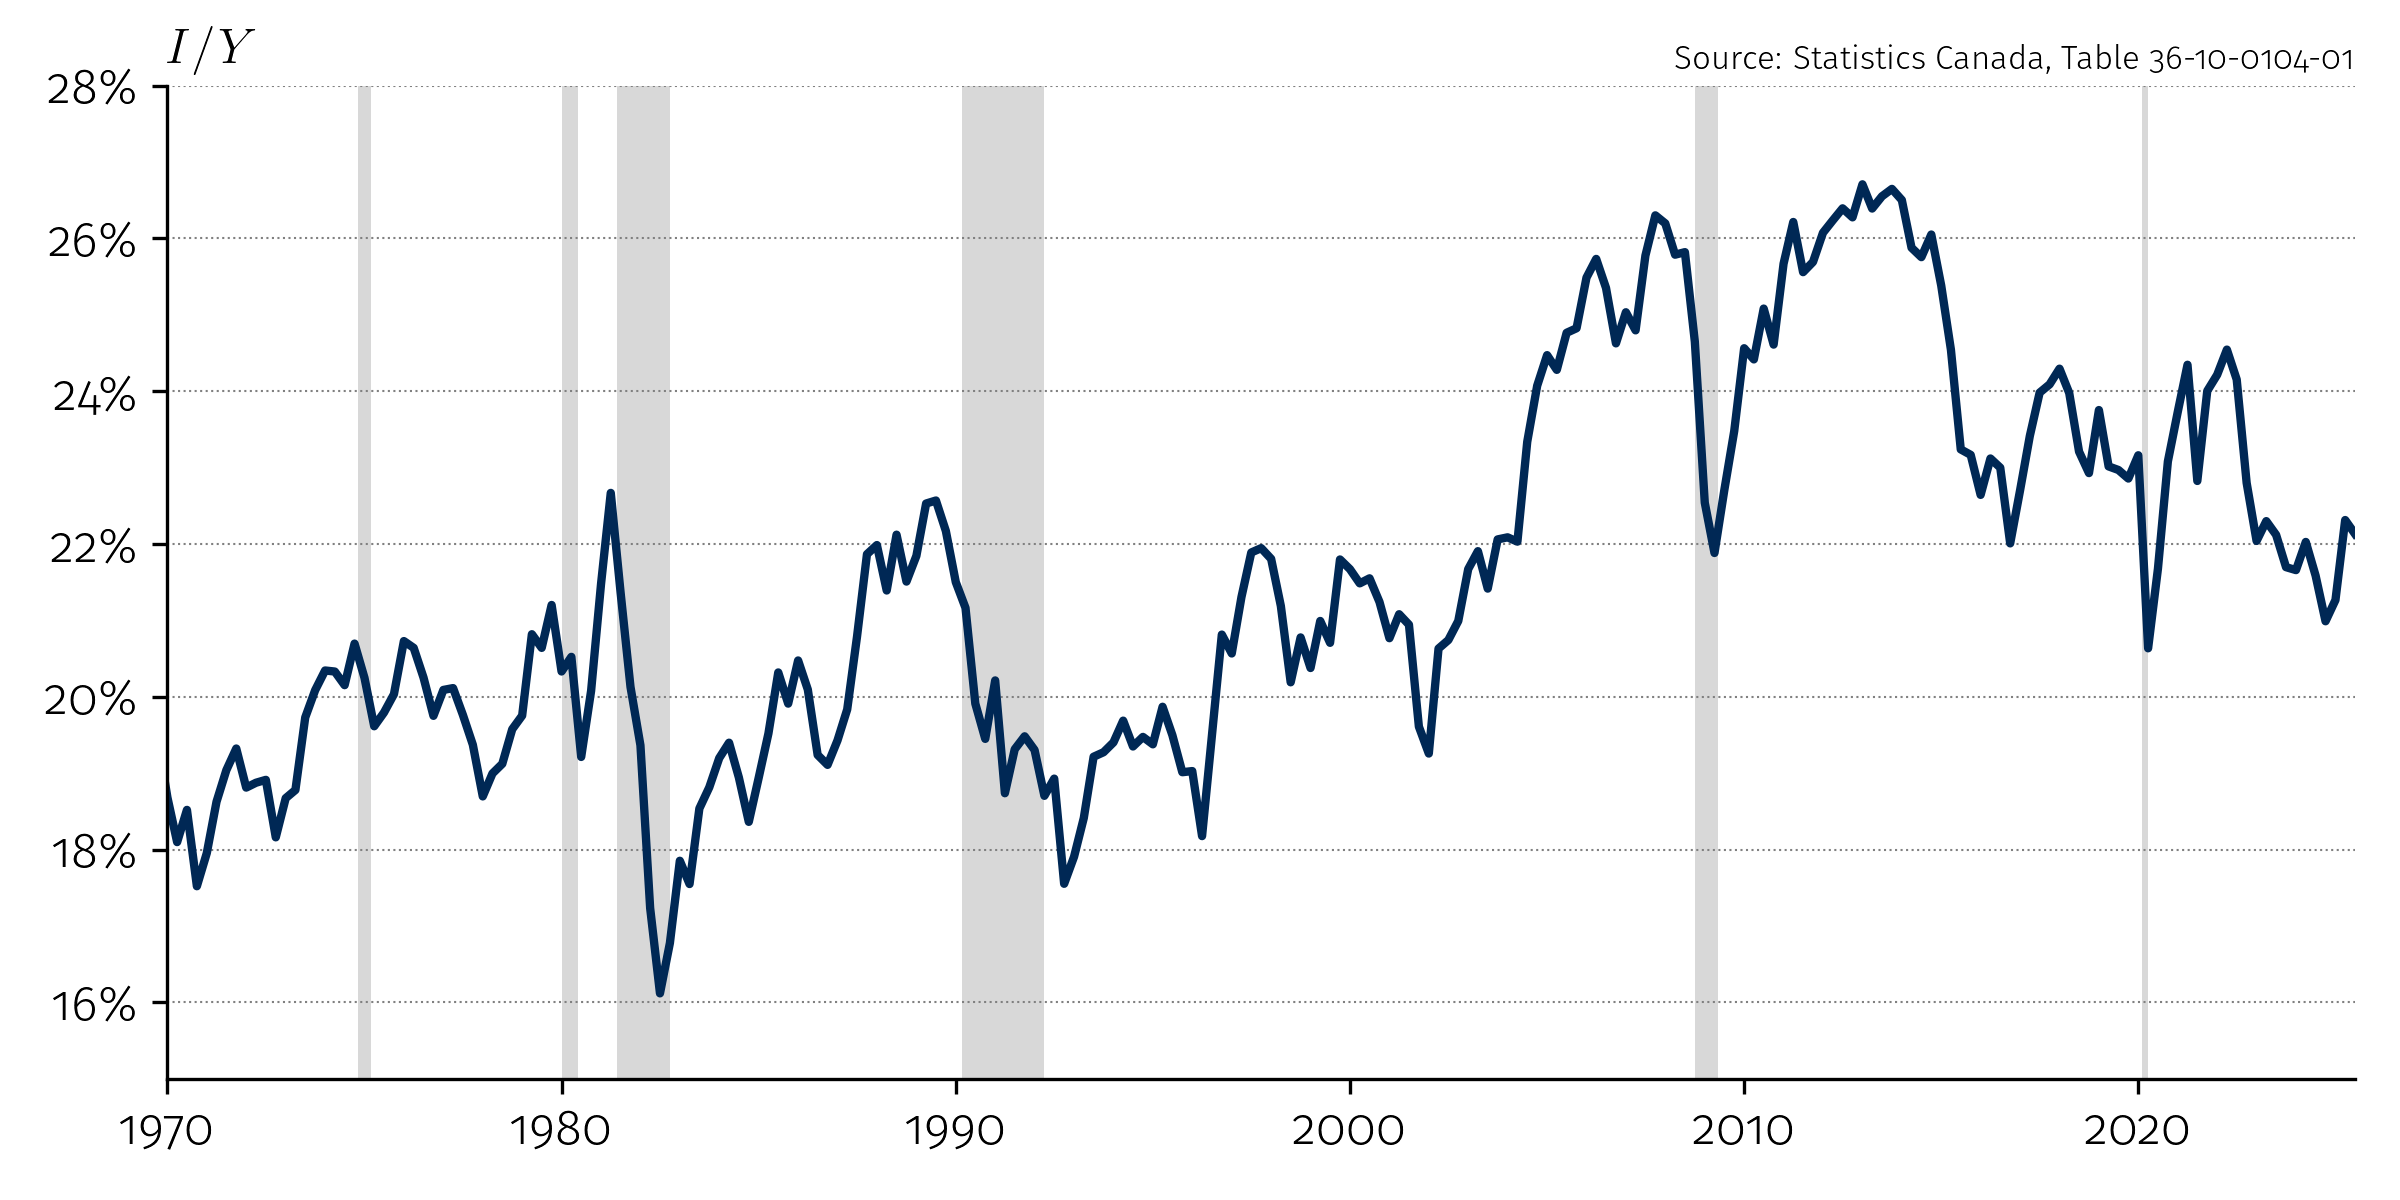
\includegraphics[width=0.95\textwidth]{investment_share_gdp.png}
   \end{figure}
   \vspace{-0.4cm}
   \footnotesize L'investissement est la composante la plus \textbf{volatile} --- il chute fortement en r\'ecession.
\end{frame}

% ── Dépenses gouvernementales ───────────────────────────────────────────────

\begin{frame}[t]{D\'epenses gouvernementales ($G$)}
   \small
   \textbf{Grand producteur} de biens/services :
   arm\'ee, \'education, sant\'e, infrastructures.
   \vspace{0.15cm}
   \begin{defbox}[\'Evalu\'e au co\^ut]
      Souvent sans prix de march\'e, donc $G$ est mesur\'e par le \textbf{co\^ut des intrants}.
   \end{defbox}
   \vspace{0.1cm}
   \begin{warning}[Transferts $\neq$ d\'epenses gouvernementales]
      Les transferts sociaux (assurance-emploi, pensions, aide sociale) ne font \textbf{pas} partie de $G$ : ils redistribuent le revenu existant, sans nouvelle production.
   \end{warning}
\end{frame}

\begin{frame}{Part de $G$ dans le PIB au Canada}
   \vspace{-0.2cm}
   \begin{figure}
      \centering
      
\includegraphics[width=0.95\textwidth]{government_share_gdp.png}
   \end{figure}
   \vspace{-0.4cm}
   \footnotesize D\'epenses publiques en hausse lors des r\'ecessions, mais en baisse tendancielle depuis les ann\'ees 1990.
\end{frame}

% ── Exportations et importations ───────────────────────────────────────────────

\begin{frame}[t]{Exportations et importations ($NX$)}
   $C$, $I$ et $G$ incluent les d\'epenses en biens \textbf{\'etrangers} (importations).\\[4pt]
   Puisque le PIB mesure la production \textit{int\'erieure}, il faut une correction :
   \vspace{0.1cm}
   \begin{equation*}
      Y = \underbrace{C + I + G}_{\text{d\'epenses totales}} + \underbrace{X - M}_{\text{export.\ nettes}}
   \end{equation*}
   \vspace{-0.3cm}
   \begin{itemize}
      \setlength\itemsep{0.1cm}
      \item $X$ (exportations) : production int\'erieure vendue \`a l'\'etranger
      \item $M$ (importations) : production \'etrang\`ere d\'ej\`a compt\'ee dans $C$, $I$, $G$
   \end{itemize}
   \vspace{0.15cm}
   \begin{defbox}[Ouverture commerciale]
      $(X + M) / Y$ mesure l'importance du commerce pour une \'economie.
   \end{defbox}
\end{frame}

\begin{frame}{Part du commerce dans le PIB au Canada}
   \vspace{-0.2cm}
   \begin{figure}
      \centering
      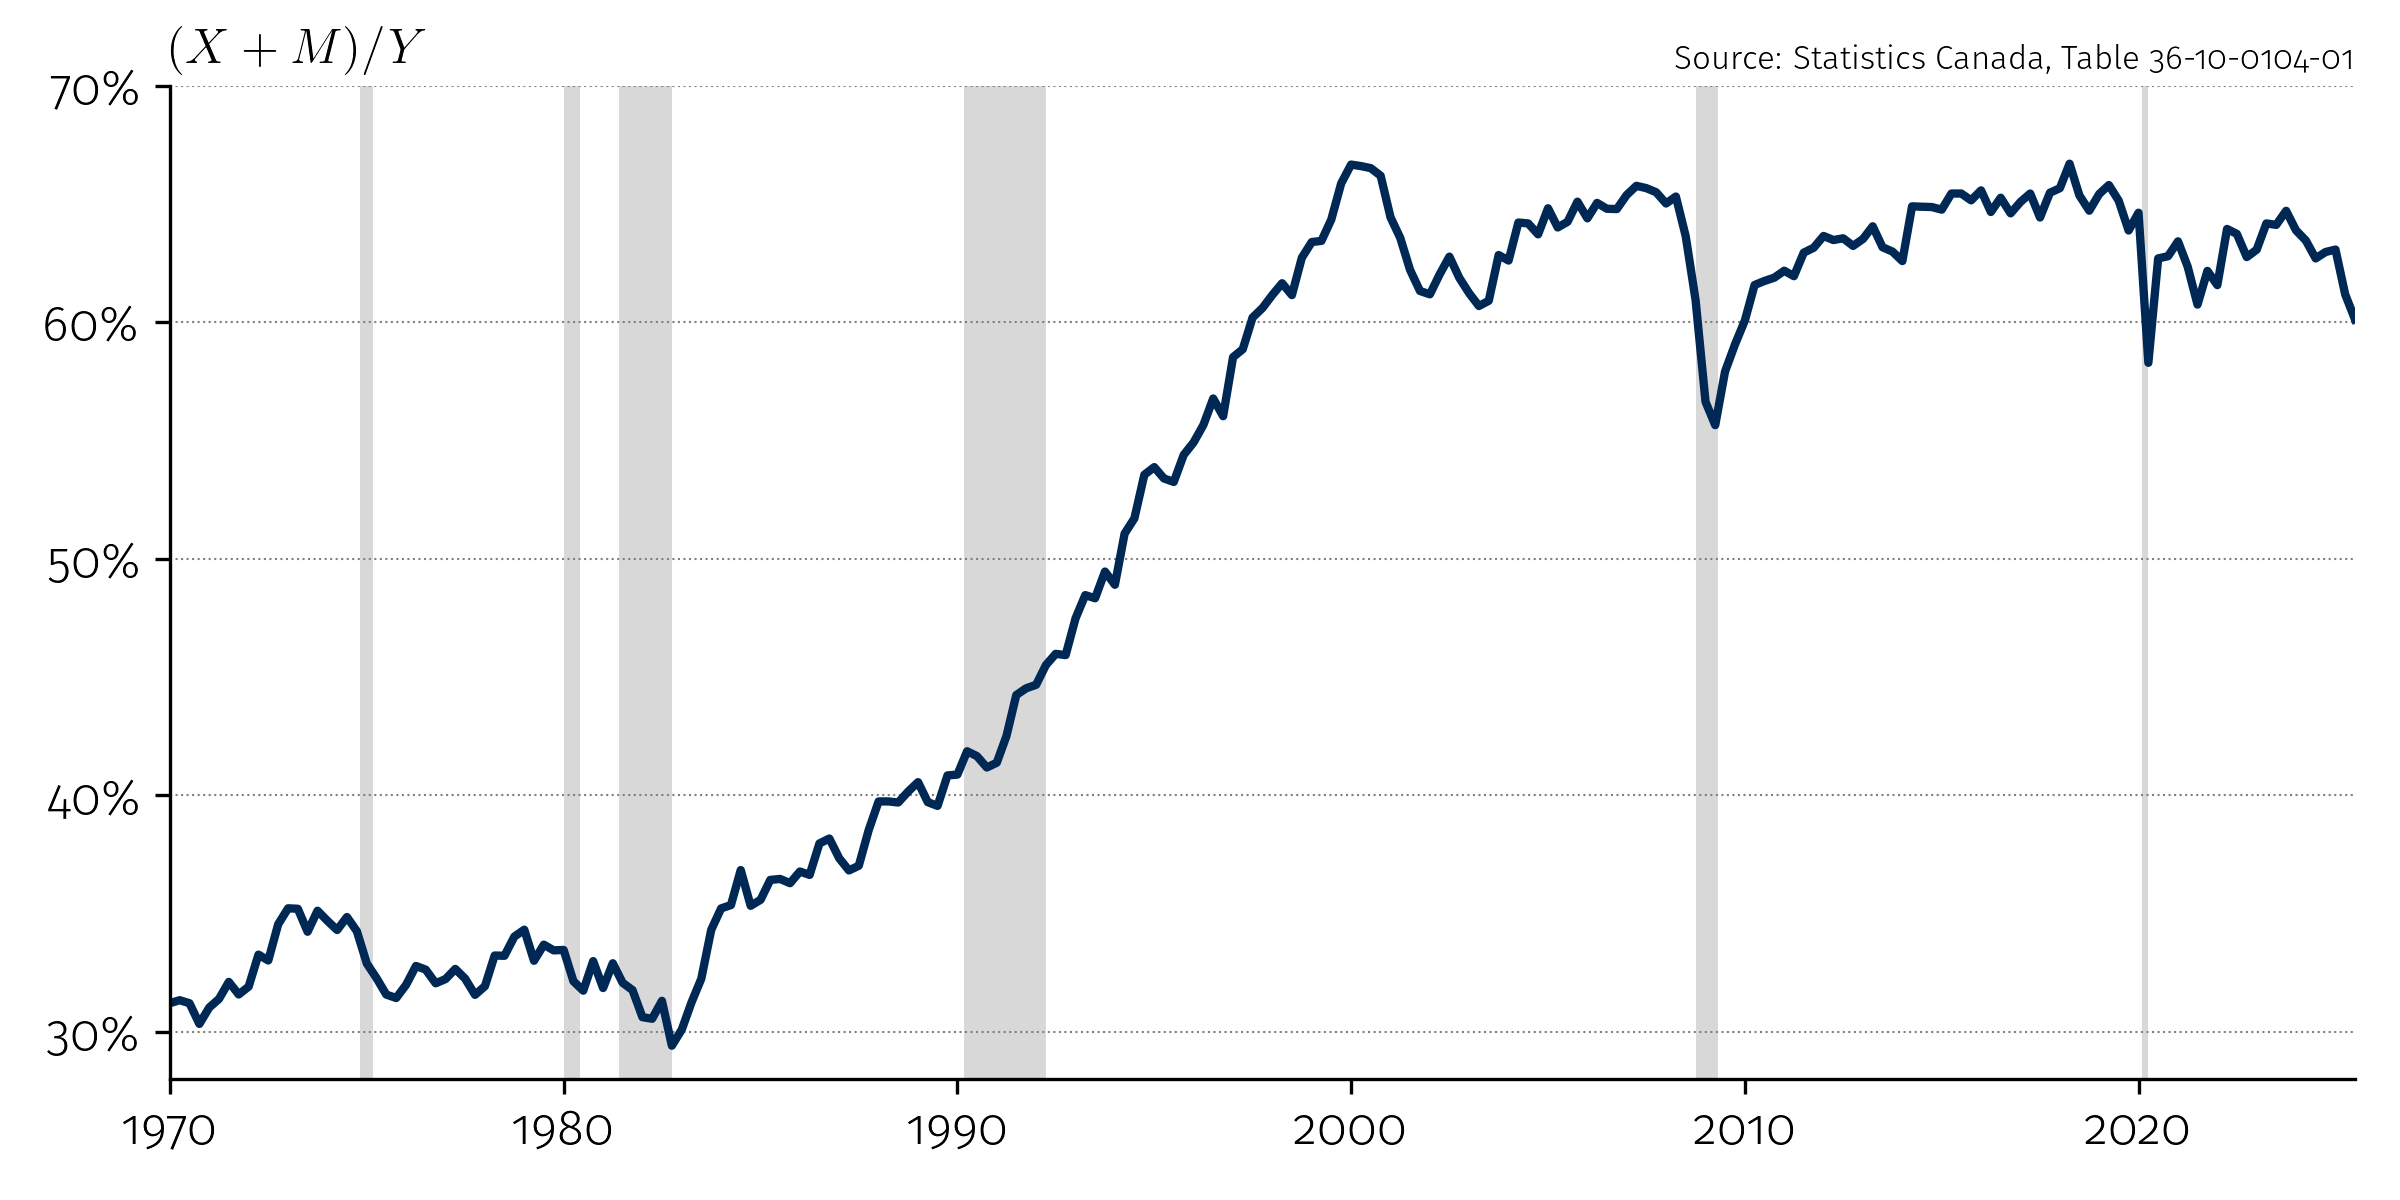
\includegraphics[width=0.95\textwidth]{trade_share_gdp.png}
   \end{figure}
   \vspace{-0.4cm}
   \footnotesize Le Canada est tr\`es ouvert. Le commerce a culmin\'e avec l'ALENA (1994), puis l\'eg\`erement diminu\'e.
\end{frame}

\begin{frame}[t]{Entra\^iner votre d\'etecteur de \guillemotleft~BS~\guillemotright}
   \footnotesize
   \vspace{0.1cm}
   \begin{columns}[T]
      \begin{column}{0.42\textwidth}
         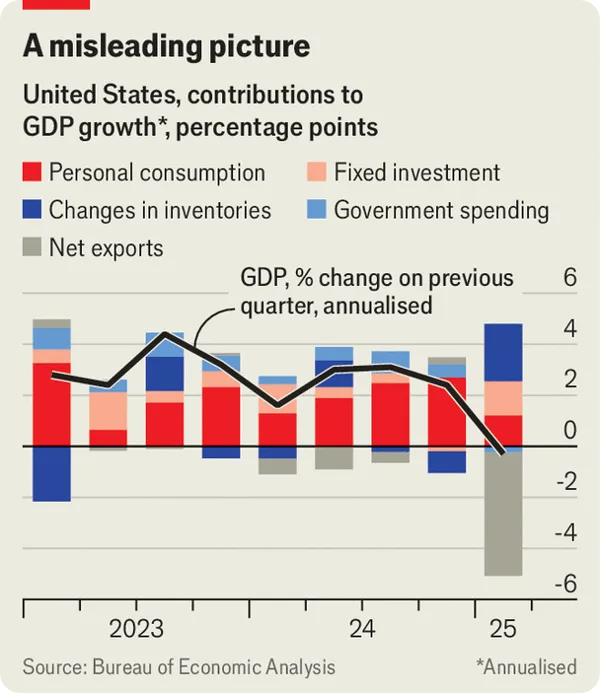
\includegraphics[width=\linewidth, height=0.65\textheight, keepaspectratio]{misleading_GDP_accounting.png}\\[-2pt]
         {\scriptsize\textcolor{HECgray}{Source: \textit{The Economist}, 2025}}
      \end{column}
      \hspace{-2cm}
      \begin{column}{0.54\textwidth}
         Au T1 2025, le PIB am\'ericain a recul\'e. On a bl\^am\'e les importations : \guillemotleft~le d\'eficit commercial a retranch\'e 5~pp \`a la croissance~\guillemotright.
         \vspace{0.15cm}
         \begin{warning}[C'est trompeur]
            \footnotesize
            Les importations entrent dans le PIB \textbf{deux fois} : \textit{ajout\'ees} dans $C$/$I$/$G$, puis \textit{soustraites} dans $NX$.\\[8pt]
            Entreprises qui devancent leurs importations avant les tarifs : $\uparrow I$, $\downarrow NX$. Les deux s'annulent.\\[8pt]
            Consommateurs qui ach\`etent avant les tarifs : $\uparrow C$, $\downarrow NX$. Les deux s'annulent.
         \end{warning}
      \end{column}
   \end{columns}
\end{frame}

\begin{frame}{PIB par les d\'epenses : comparaison internationale}
   \vspace{-0.15cm}
   \begin{figure}
      \centering
      
\includegraphics[width=\textwidth, height=0.62\textheight, keepaspectratio]{gdp_decomposition_4countries.png}
   \end{figure}
   \vspace{-0.25cm}
   \begin{keyinsight}[Diff\'erents mod\`eles de croissance]
      Chine : investissement ($I$ = 41\,\%). \'E.-U.\ : consommation ($C$ = 68\,\%). Ces diff\'erences fa\c{c}onnent \'echanges et strat\'egies.
   \end{keyinsight}
\end{frame}

\begin{frame}[t]{Ce que le PIB ne mesure \textit{pas}}
   Le PIB ne comptabilise que les \textbf{transactions marchandes}. Beaucoup d'activit\'e \'economique est omise :
   \vspace{0.2cm}
   \begin{itemize}
      \setlength\itemsep{0.15cm}
      \item \textbf{Production domestique} --- cuisine, garde d'enfants, r\'eparations \`a domicile
      \item \textbf{B\'en\'evolat} --- services communautaires, organismes de bienfaisance
      \item \textbf{\'Economie souterraine} --- revenus non d\'eclar\'es, travail informel
   \end{itemize}
   \vspace{0.2cm}
   \begin{keyinsight}[Sexe, drogues et PIB]
      En 2014, l'UE a exig\'e l'inclusion des activit\'es ill\'egales (drogues, prostitution) dans le PIB. Le PIB de l'Italie a bondi de 18\,\% du jour au lendemain\ldots
      \hfill{\scriptsize\textit{\color{black!50}The Economist, 2014}}
   \end{keyinsight}
\end{frame}

\begin{frame}{Peut-on se fier aux chiffres du PIB?}
   \centering
   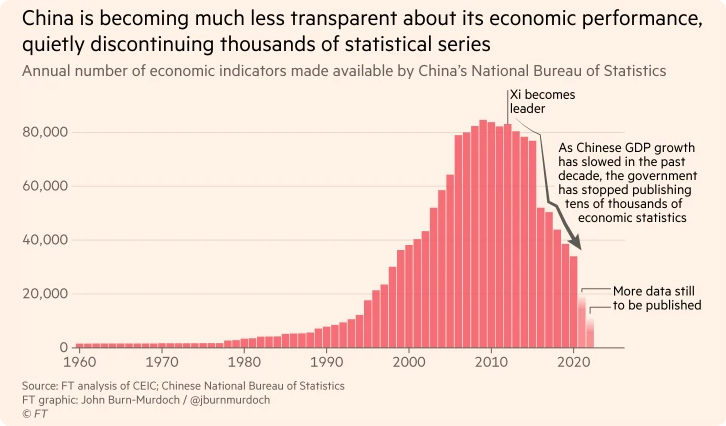
\includegraphics[height=0.75\textheight, keepaspectratio]{china_transparency.png}
\end{frame}

\begin{frame}[t]{Manipulation du PIB : trois mises en garde}
   \small
   \begin{itemize}
      \setlength\itemsep{0.1cm}
      \item \textbf{Chine :} croissance suspecte de r\'egularit\'e, s\'eries de plus en plus discontinu\'ees, provinces alignant leurs chiffres sur les cibles centrales\ldots Les autocraties surestiment la croissance de $\sim$35\,\% en moyenne.
         \\{\scriptsize\textcolor{HECgray}{Martinez, ``How Much Should We Trust the Dictator's GDP Growth Estimates?'' \textit{JPE}, 2022}}
      \item \textbf{Venezuela :} banque centrale muette sur le PIB et l'inflation de 2016 \`a 2019; \`a la reprise, elle a r\'ev\'el\'e une contraction cumulative de $\sim$47\,\%
         \\{\scriptsize\textcolor{HECgray}{IMF World Economic Outlook; Banco Central de Venezuela, 2019}}
      \item \textbf{Gr\`ece :} d\'eficit 2009 d\'eclar\'e \`a 3,7\,\% du PIB, r\'evis\'e \`a 15,4\,\% --- 4$\times$ le chiffre initial, d\'eclenchant la crise de la dette europ\'eenne
         \\{\scriptsize\textcolor{HECgray}{European Commission, Report on Greek Government Deficit and Debt Statistics, 2010}}
   \end{itemize}
   \begin{bizimplication}[V\'erification diligente]
      \footnotesize Ne prenez pas le PIB officiel pour argent comptant. Recoupez avec des donn\'ees alternatives --- surtout dans les autocraties.
   \end{bizimplication}
\end{frame}

\begin{frame}[t]{Quand les donn\'ees manquent\ldots les \'economistes s'inventent!}
   \footnotesize
   \begin{itemize}
      \setlength\itemsep{0.3cm}
      \item \textbf{Lumi\`eres nocturnes par satellite :} luminosit\'e $\approx$ activit\'e \'economique --- aussi informatif que le PIB officiel pour les pays aux donn\'ees lacunaires,
         {\scriptsize\textcolor{HECgray}{(Henderson et al., \textit{AER}, 2012).}}
      \item \textbf{Donn\'ees portuaires :} volumes d'exp\'edition, tirant d'eau AIS, douanes, d\'ebit de conteneurs r\'ev\`elent des flux que les statistiques sous-estiment.
      \item \textbf{Apprentissage automatique :} algorithmes d\'etectant les p\'etroliers qui coupent leurs transpondeurs pour contourner les sanctions (\guillemotleft~dark shipping~\guillemotright),
         {\scriptsize\textcolor{HECgray}{(Fern\'andez-Villaverde et al., NBER WP 33486, 2025).}}
      \item \textbf{Prix en ligne :} prix de d\'etail collect\'es sur le web, suivant l'inflation au quotidien --- ont r\'ev\'el\'e la manipulation de l'IPC argentin,
         {\scriptsize\textcolor{HECgray}{(Cavallo \& Rigobon, \textit{JEP}, 2016).}}
      \item \textbf{T\'el\'ephonie mobile :} densit\'e des appels et achats de temps d'antenne $\approx$ consommation dans les pays en d\'eveloppement.
   \end{itemize}
\end{frame}

\begin{frame}{Quand l'obscurit\'e \'eclaire\ldots}
   \centering
   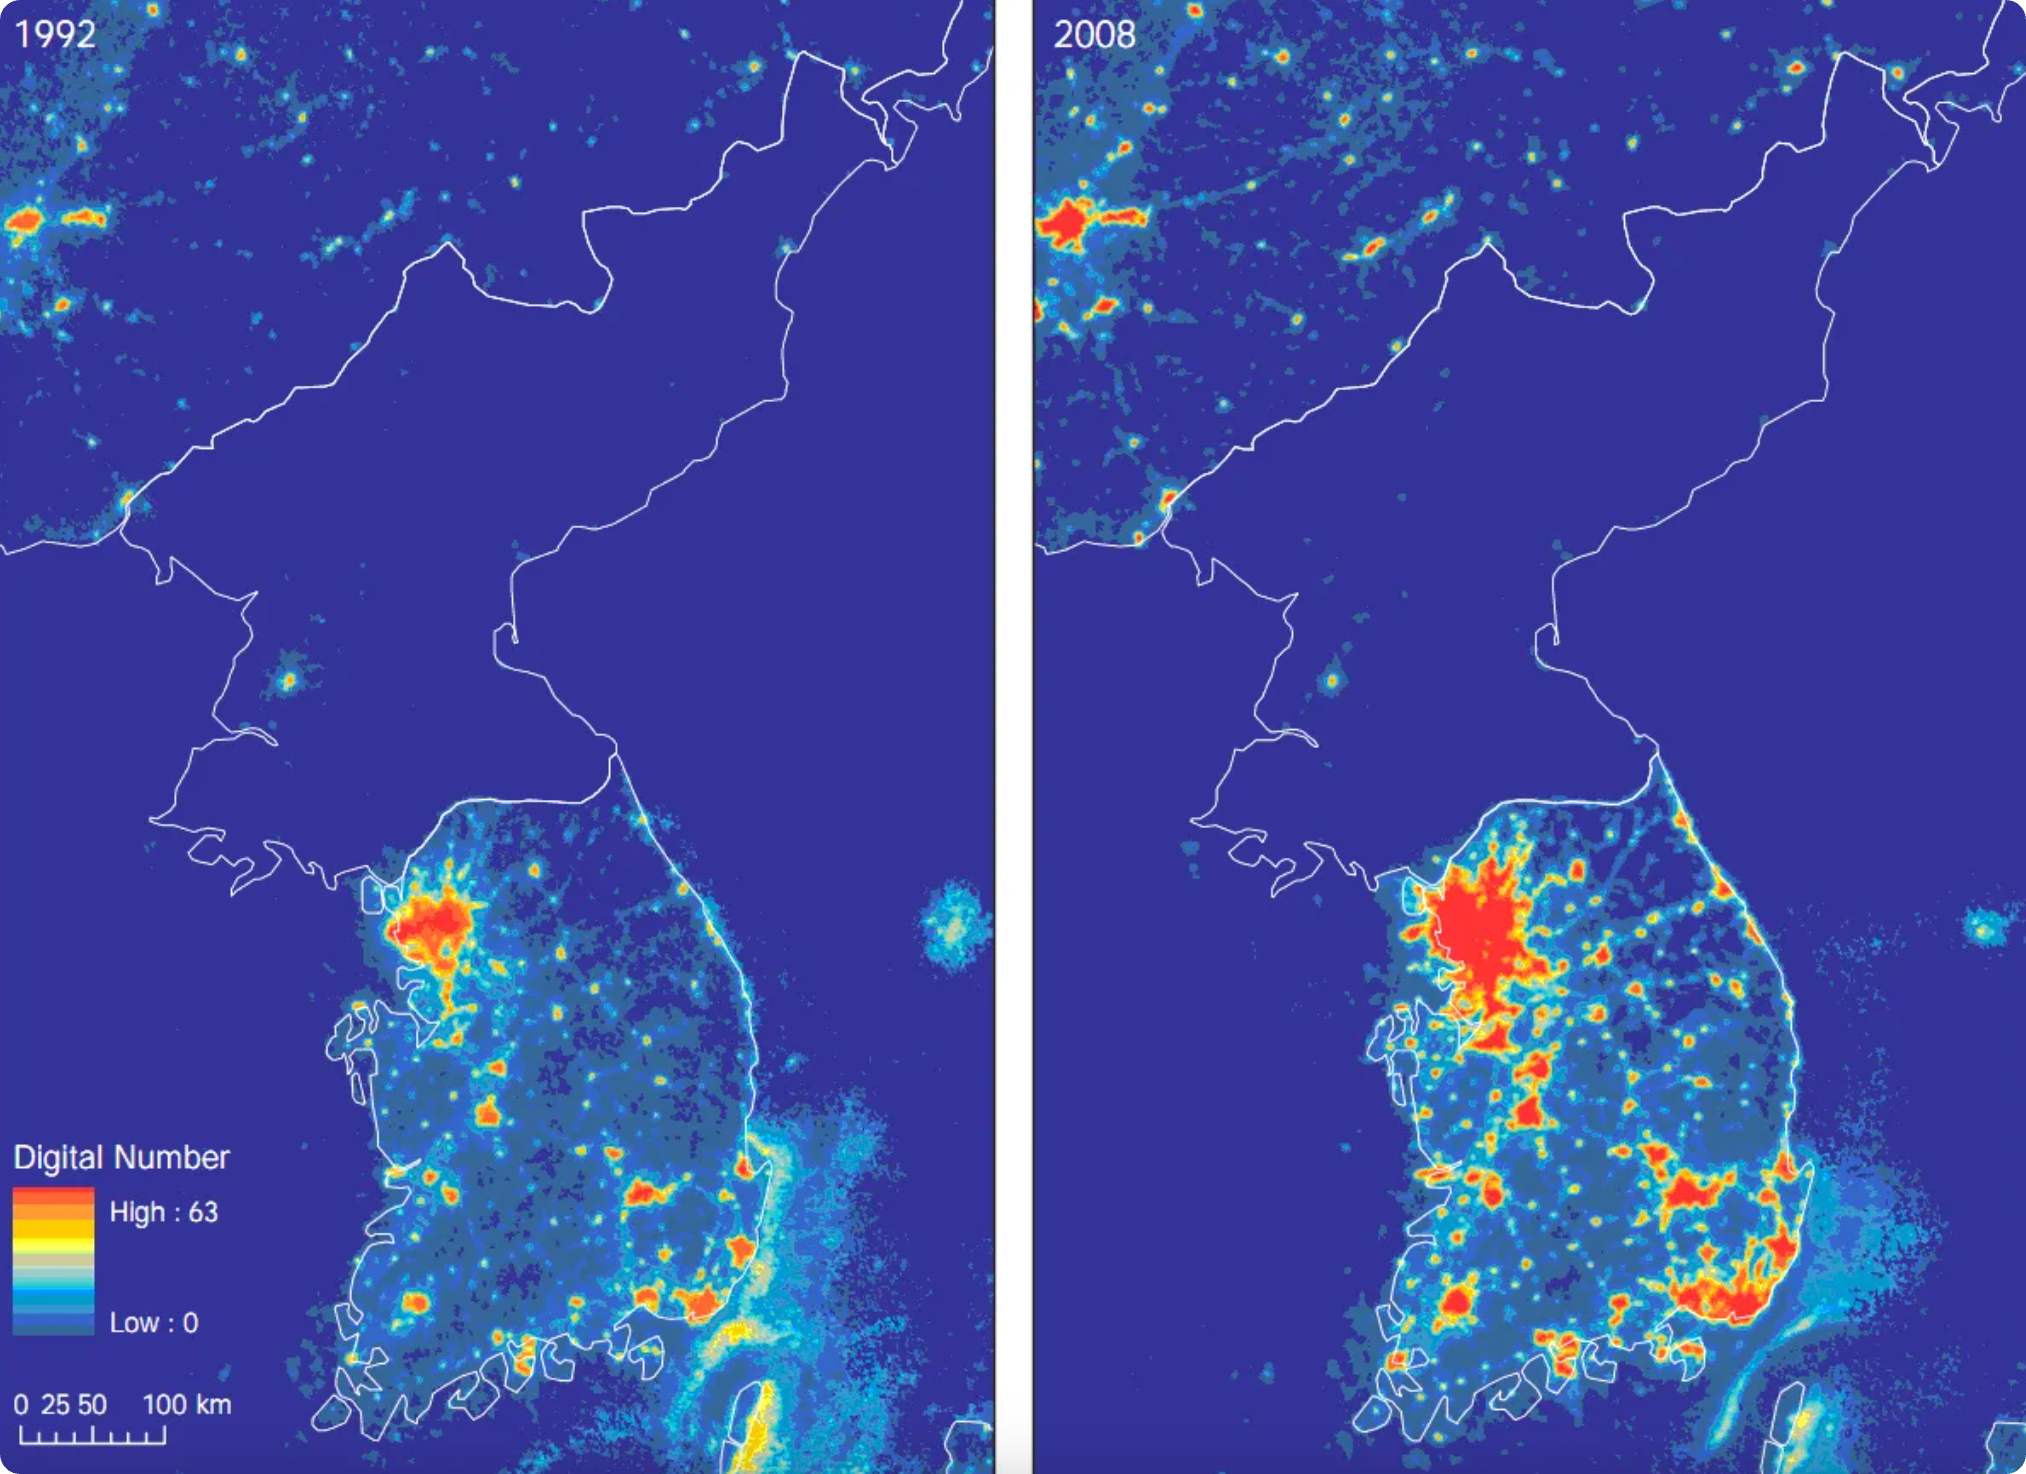
\includegraphics[height=0.75\textheight, keepaspectratio]{korea_space.png}
\end{frame}

\begin{frame}[t]{Quand l'obscurit\'e \'eclaire\ldots}
   \centering
   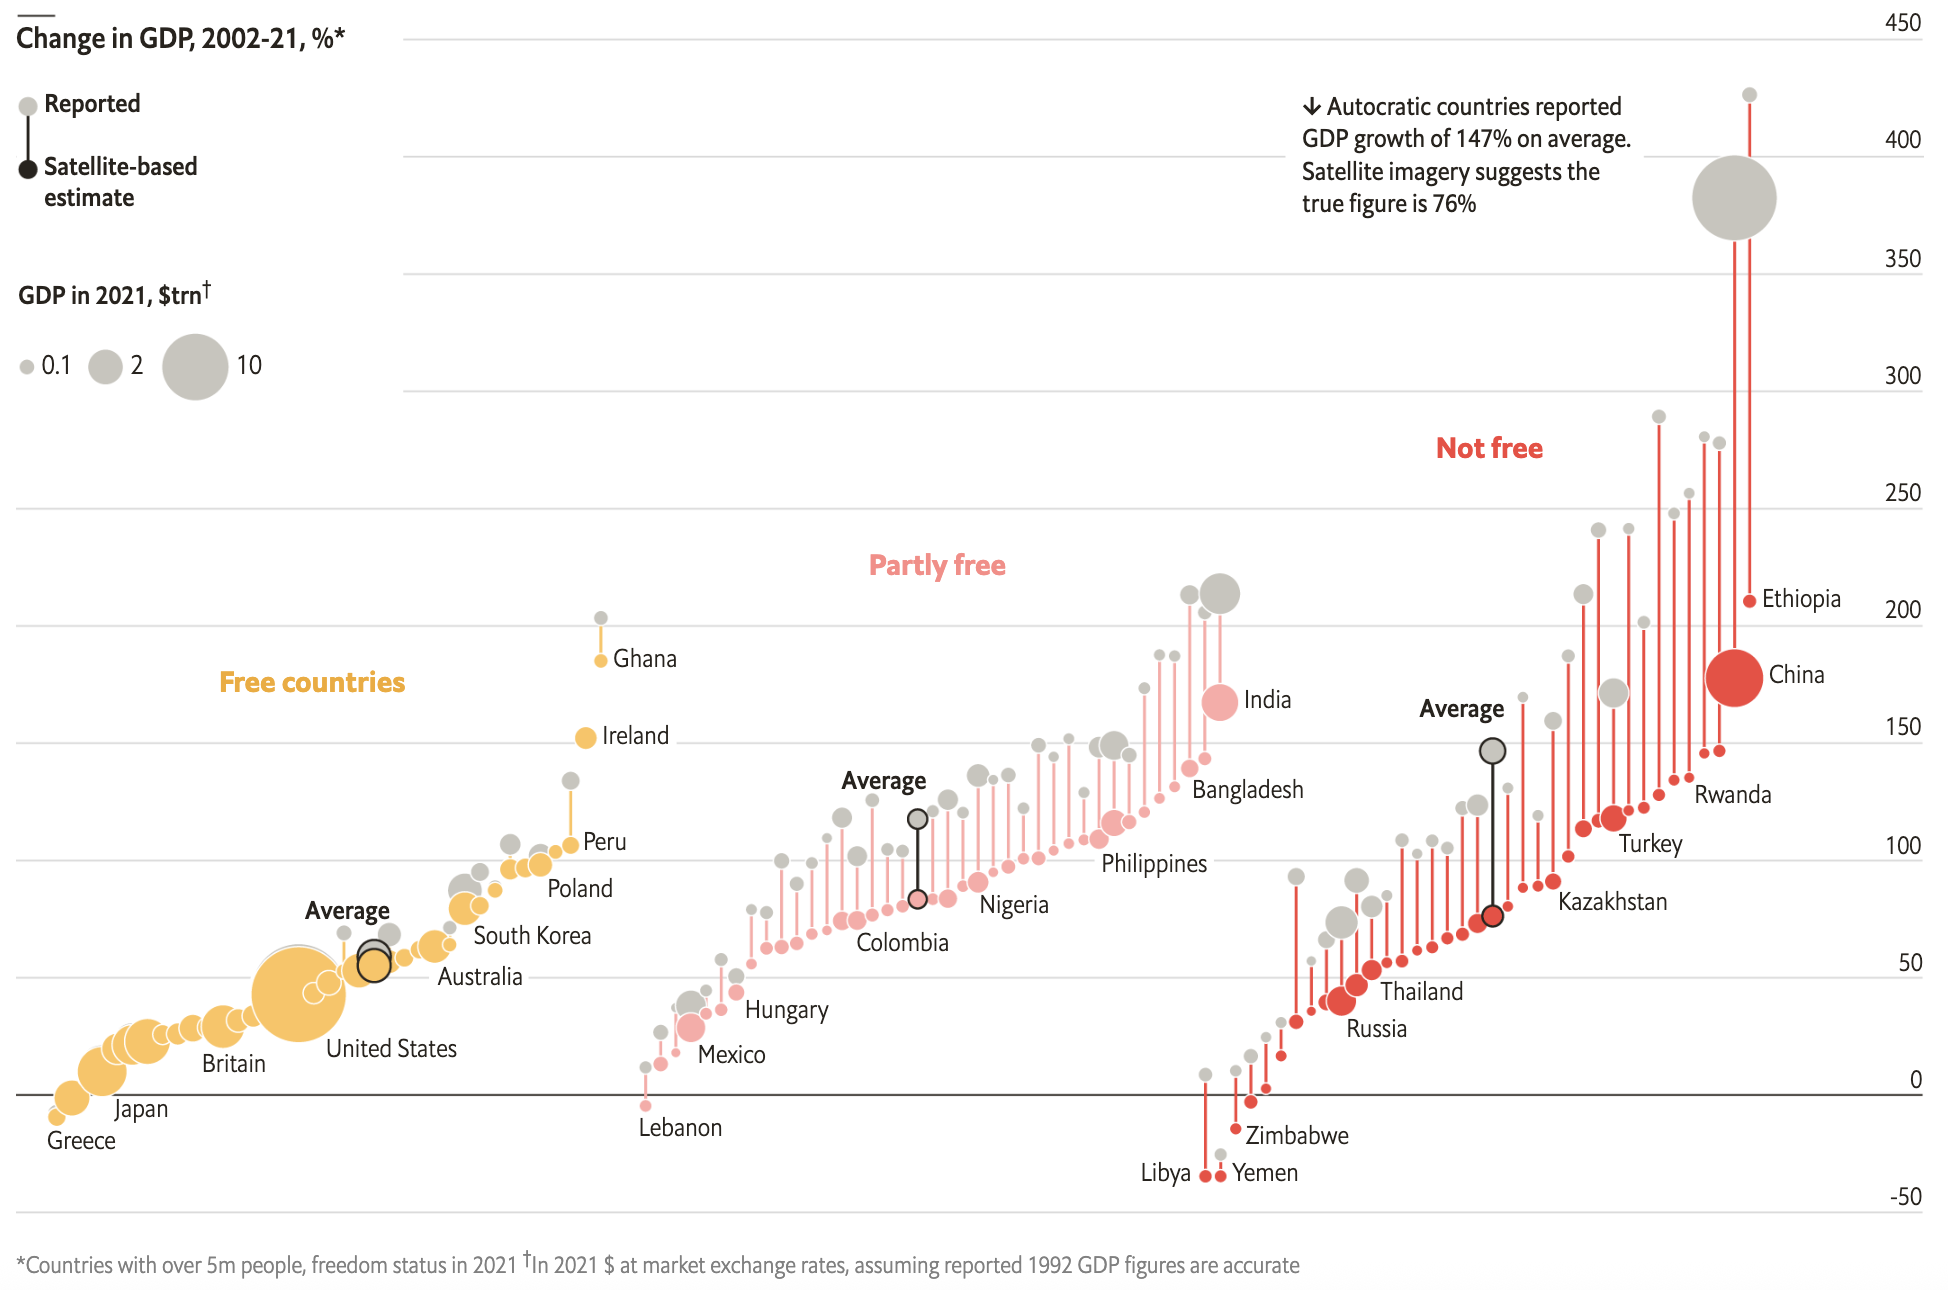
\includegraphics[height=0.8\textheight, keepaspectratio]{gdp_manipulation.png}
\end{frame}

% ============================================================================
\begin{frame}{Plan}
   \begin{enumerate}
      \setlength\itemsep{0.35cm}
      \item {\color{gray!50}Aper\c{c}u du cours et logistique}
      \item {\color{gray!50}Mesurer l'\'economie : le PIB}
      \item \textbf{Comparer le PIB dans le temps}
      \item Comparer le PIB entre pays
      \item Au-del\`a du PIB
   \end{enumerate}
\end{frame}

% ============================================================================
\sectionframe{Comparer le PIB dans le temps}
% ============================================================================

\begin{frame}{Croissance du PIB nominal au Canada}
   \begin{figure}
      \centering
      
\includegraphics[width=\textwidth]{gdp_nominal_canada.png}
   \end{figure}
\end{frame}

\begin{frame}{Croissance du PIB nominal vs.\ r\'eel au Canada}
   \begin{figure}
      \centering
      
\includegraphics[width=\textwidth]{gdp_nominal_real_canada.png}
   \end{figure}
\end{frame}

\begin{frame}[t]{PIB et prix}
   \begin{defbox}
      \vspace{-0.5cm}
      \begin{itemize}
         \setlength\itemsep{0.15cm}
         \item \textbf{PIB nominal} = production \'evalu\'ee aux prix \textit{courants}
         \item \textbf{PIB r\'eel} = production \'evalu\'ee aux prix \textit{constants}
         \item \textbf{D\'eflateur du PIB} = $\frac{\text{PIB nominal}}{\text{PIB r\'eel}} \times 100$
      \end{itemize}
   \end{defbox}
   \vspace{0.05cm}
   \begin{keyinsight}
      Le PIB nominal est biais\'e par les variations de prix. Le PIB r\'eel isole les variations de quantit\'e, mesurant la vraie croissance.
   \end{keyinsight}
\end{frame}

\begin{frame}[t]{Et si la hausse des prix refl\`ete une meilleure qualit\'e?}
   \small
   Quand un bien/service \textbf{s'am\'eliore}, une partie de la hausse de prix refl\`ete la qualit\'e, pas l'inflation :
   \vspace{0.15cm}
   \begin{itemize}
      \setlength\itemsep{0.15cm}
      \item \textbf{Voitures neuves :} prix moyen de $\sim$23K\,\$ (2005) \`a $\sim$48K\,\$ (2024) --- mais 10+ coussins gonflables, aide au maintien de voie, cam\'era de recul, dur\'ee de vie doubl\'ee
      \item \textbf{M\'edicaments anticancer :} de $\sim$10K\,\$/an (2000) \`a $>$100K\,\$ (immunoth\'erapies) --- mais mortalit\'e par cancer $-$34\,\% depuis 1991
   \end{itemize}
   \vspace{0.1cm}
   \begin{keyinsight}
      Les agences statistiques ajustent pour cela (\textbf{prix h\'edoniques}), mais la vraie am\'elioration de qualit\'e est $\sim$\textbf{3$\times$} ce qu'elles mesurent. Surestimer l'inflation = sous-estimer la croissance du PIB r\'eel\ldots
      \hfill{\scriptsize\textcolor{HECgray}{Bils \& Klenow, \textit{AER}, 2001}}
   \end{keyinsight}
\end{frame}

\begin{frame}{L'inflation est de retour\ldots}
   \begin{tikzpicture}[remember picture, overlay]
      \setcounter{newshl}{0}
      \newsheadline[bloomberg]{Bloomberg}{``The Affordability Crisis Should Have Been Over By Now''}
      \newsheadline[washpost]{The Washington Post}{``Rising prices fueled by tariffs, delayed inflation report shows''}
      \newsheadline[globeandmail]{The Globe and Mail}{``Canada's inflation rate rises to 2.4\% as grocery prices surge''}
      \newsheadline[ledevoir]{Le Devoir}{``Vers une nouvelle hausse du prix des aliments en 2026''}
      \newsheadline[wsj]{The Wall Street Journal}{``Trump's Tariffs Cost the Average Household \$1,000 Last Year''}
      \newsheadline[lapresse]{La Presse}{``L'inflation alimentaire ne dispara\^itra pas de sit\^ot''}
   \end{tikzpicture}
\end{frame}

\begin{frame}{Qu'est-ce que l'inflation?}
   \begin{defbox}[Inflation]
      Le taux de variation en \% du \textbf{niveau g\'en\'eral des prix} entre deux p\'eriodes.
   \end{defbox}

   \begin{equation*}
      \pi_t = \frac{P_t - P_{t-1}}{P_{t-1}} = \%\Delta P \quad \text{o\`u $P_t =$ niveau des prix au temps $t$}
   \end{equation*}

   \vspace{0.3cm}

   \textbf{Question cl\'e :} comment mesurer $P_t$?
   \vspace{0.2cm}
   \begin{itemize}
      \setlength\itemsep{0.15cm}
      \item \textbf{D\'eflateur du PIB :} prix de tous les biens produits domestiquement (large)
      \item \textbf{Indice des prix \`a la consommation (IPC) :} prix d'un panier de biens de consommation (le plus courant)
   \end{itemize}
\end{frame}

\begin{frame}{Inflation r\'ecente au Canada}
   \begin{figure}
      \centering
      
\includegraphics[width=0.95\textwidth, height=0.75\textheight, keepaspectratio]{inflation_cpi_deflator_canada.png}
   \end{figure}
\end{frame}

\begin{frame}{Inflation globale vs.\ de base}
   \begin{figure}
      \centering
      
\includegraphics[width=0.95\textwidth, height=0.75\textheight, keepaspectratio]{inflation_headline_core_canada.png}
   \end{figure}
\end{frame}

\begin{frame}[t]{Indicateurs d'inflation \`a haute fr\'equence}
   \small
   Collecter \textbf{des millions de prix en ligne chaque jour} : alternative en temps r\'eel \`a l'IPC officiel
   \vspace{0.1cm}
   \begin{figure}
      \centering
      
\includegraphics[width=0.92\textwidth, height=0.72\textheight, keepaspectratio]{inflation_highfreq_cavallo.png}
   \end{figure}
\end{frame}

\begin{frame}[t]{Biais des nouveaux produits et le prix de la lumi\`ere}
   \small
   Quand un produit \textbf{nouveau} appara\^it, il n'a pas de pr\'ed\'ecesseur. L'indice de prix recommence \`a z\'ero, ratant le bond\ldots
   \vspace{0.25cm}
   \begin{keyinsight}[Le prix de la lumi\`ere (Nordhaus, 1997)]
      \vspace{-0.5cm}
      \begin{itemize}
         \item Qu'achetons-nous avec une bougie, une lampe \`a k\'eros\`ene, une ampoule?
         \item Nous achetons de la \textbf{lumi\`ere} --- des lumens!
         \item Des bougies aux DEL, le vrai co\^ut par lumen a \'et\'e divis\'e par $\sim$500.
         \item Mais les prix suivent les \textbf{produits} (bougies, lampes), pas les lumens.
         \item Chaque saut technologique \textbf{r\'einitialise} la comparaison --- la r\'evolution est invisible.
      \end{itemize}
   \end{keyinsight}
\end{frame}

% ============================================================================
\begin{frame}{Plan}
   \begin{enumerate}
      \setlength\itemsep{0.35cm}
      \item {\color{gray!50}Aper\c{c}u du cours et logistique}
      \item {\color{gray!50}Mesurer l'\'economie : le PIB}
      \item {\color{gray!50}Comparer le PIB dans le temps}
      \item \textbf{Comparer le PIB entre pays}
      \item Au-del\`a du PIB
   \end{enumerate}
\end{frame}

% ============================================================================
\sectionframe{Comparer le PIB entre pays}
% ============================================================================

\begin{frame}{L'\'economie mondiale en un coup d'\oe il}
   \vspace{-0.2cm}
   \begin{figure}
      \centering
      
\includegraphics[width=\textwidth, height=0.75\textheight, keepaspectratio]{gdp_ppp_world.png}
   \end{figure}
   \vspace{-0.3cm}
   \footnotesize La Chine a d\'epass\'e les \'E.-U.\ en termes de PPA --- mais que signifie \guillemotleft~PPA~\guillemotright?
\end{frame}

\begin{frame}[t]{Comment g\'erer des unit\'es diff\'erentes?}
   \framesubtitle{Pourquoi les taux de change peuvent \^etre trompeurs}
   \small

   \textbf{Deux fa\c{c}ons de convertir le PIB en devise commune :}
   \vspace{0.15cm}
   \begin{enumerate}
      \setlength\itemsep{0.15cm}
      \item \textbf{Taux de change du march\'e :}  $\smallquad e^N = \mathdollar_D / \mathdollar_F$
      \vspace{0.1cm}
      \begin{itemize}
         \setlength\itemsep{0.1cm}
         \item Largement disponibles et mis \`a jour fr\'equemment
         \item Probl\`eme : tr\`es volatils, et ignorent les diff\'erences de niveaux de prix
      \end{itemize}
      \item \textbf{Parit\'e de pouvoir d'achat (PPA) :} $\smallquad e^{PPA} = P_D / P_F$
      \vspace{0.1cm}
      \begin{itemize}
         \setlength\itemsep{0.1cm}
         \item Meilleures comparaisons de niveaux de vie : un dollar ach\`ete plus \`a Lagos qu'\`a New York
         \item Les biens/services sont-ils comparables d'un pays \`a l'autre?
         \item Mis \`a jour moins fr\'equemment
         \item Taux de change r\'eel : $e^R = e^N / e^{PPA}$
      \end{itemize}
   \end{enumerate}
\end{frame}

\begin{frame}{Prix plus \'elev\'es dans les pays riches (effet Balassa-Samuelson)}
   \vspace{-0.2cm}
   \begin{figure}
      \centering
      
\includegraphics[width=\textwidth, height=0.8\textheight, keepaspectratio]{gdp_per_capita_vs_price_level.png}
   \end{figure}
\end{frame}

\begin{frame}[t]{L'indice Big Mac}
   \small
   \vspace{-0.1cm}
   \begin{columns}[T]
      \begin{column}{0.6\textwidth}
         \begin{figure}
            \centering
            
\includegraphics[width=\textwidth, height=0.82\textheight, keepaspectratio]{big_mac_index.png}
         \end{figure}
      \end{column}
      \begin{column}{0.37\textwidth}
         Un Big Mac est (grosso modo) le m\^eme produit partout $\to$ mesure PPA \guillemotleft~rapide et approximative~\guillemotright
         \vspace{0.2cm}

         \textbf{Exemple (Suisse) :}
         \vspace{0.05cm}
         \begin{itemize}
            \setlength\itemsep{0.05cm}
            \footnotesize
            \item En Suisse : 6,90 CHF
            \item Aux \'E.-U.\ : 5,69\,\$
            \item PPA implicite : $\frac{6{,}90}{5{,}69} = 1{,}21 \text{ CHF} / \mathdollar$
            \item Taux du march\'e $\approx 0{,}88 \text{ CHF} / \mathdollar$
            \item Le CHF est \textbf{sur\'evalu\'e}
         \end{itemize}
         \vspace{0.15cm}
         {\footnotesize Publi\'e par \textit{The Economist} depuis 1986 --- mi-s\'erieux, mi-amusant}
      \end{column}
   \end{columns}
\end{frame}

\begin{frame}[t]{PIB r\'eel vs.\ PIB r\'eel par habitant}
   \small
   \begin{itemize}
      \setlength\itemsep{0.15cm}
      \item Le \textbf{PIB r\'eel} mesure la taille totale de l'\'economie
      \item Le \textbf{PIB r\'eel par habitant} mesure le niveau de vie moyen
   \end{itemize}
   \vspace{0.1cm}
   \begin{bizimplication}[Strat\'egie de march\'e]
      \small Vous vendez des sacs \`a main de luxe. Viser un pays au PIB \'elev\'e ou au PIB par habitant \'elev\'e? Et si vous vendez des biens abordables \`a faibles marges?
   \end{bizimplication}
   \vspace{0.1cm}
   \begin{bizimplication}[R\'emun\'eration]
      \small Vos employ\'es demandent une hausse car \guillemotleft~l'\'economie cro\^it~\guillemotright. Le PIB a progress\'e de 15\,\% en 10 ans. Bon argument pour de meilleurs salaires?
   \end{bizimplication}
\end{frame}

\begin{frame}{Le Canada suit le rythme des \'Etats-Unis\ldots}
   \begin{figure}
      \centering
      
\includegraphics[width=\textwidth]{gdp_canada_usa.png}
   \end{figure}
\end{frame}

\begin{frame}{Jusqu'\`a ce qu'on ajuste pour la d\'emographie\ldots}
   \begin{figure}
      \centering
      
\includegraphics[width=\textwidth]{gdp_per_capita_canada_usa.png}
   \end{figure}
\end{frame}

\begin{frame}{PIB vs.\ PIB par habitant \`a travers le monde}
   \vspace{-0.2cm}
   \begin{figure}
      \centering
      
\includegraphics[width=\textwidth, height=0.78\textheight, keepaspectratio]{gdp_vs_gdp_per_capita.png}
   \end{figure}
   \vspace{-0.3cm}
   \footnotesize Grande \'economie $\neq$ population riche. L'Inde et la Chine ont un PIB massif mais un PIB par habitant modeste.
\end{frame}

% ============================================================================
\begin{frame}{Plan}
   \begin{enumerate}
      \setlength\itemsep{0.35cm}
      \item {\color{gray!50}Aper\c{c}u du cours et logistique}
      \item {\color{gray!50}Mesurer l'\'economie : le PIB}
      \item {\color{gray!50}Comparer le PIB dans le temps}
      \item {\color{gray!50}Comparer le PIB entre pays}
      \item \textbf{Au-del\`a du PIB}
   \end{enumerate}
\end{frame}

% ============================================================================
\sectionframe{Au-del\`a du PIB}
% ============================================================================

\begin{frame}[t]{Ce que le PIB ne capte pas}
   \small
   Le PIB est utile mais incomplet. Il omet :
   \vspace{0.1cm}
   \begin{itemize}
      \setlength\itemsep{0.05cm}
      \item \textbf{In\'egalit\'es :} le PIB peut cro\^itre m\^eme si la majorit\'e s'appauvrit
      \item \textbf{Loisir :} travailler 80h/sem.\ augmente le PIB, pas le bien-\^etre
      \item \textbf{Sant\'e :} esp\'erance de vie, sant\'e mentale, morbidit\'e
      \item \textbf{Environnement :} pollution, \'epuisement des ressources, climat
      \item \textbf{Libert\'e politique :} d\'emocratie, droits de la personne, corruption
      \item \textbf{S\'ecurit\'e :} criminalit\'e, conflits
   \end{itemize}
   \vspace{0.05cm}
   \begin{bizimplication}[ESG et parties prenantes]
      \footnotesize Investisseurs et consommateurs \'evaluent de plus en plus les entreprises sur des dimensions hors PIB. Comprendre ces limites aide \`a anticiper la r\'eglementation.
   \end{bizimplication}
\end{frame}

\begin{frame}{}
   \small
   \begin{quotation}
      Our gross national product, now, is over \$800 billion dollars a year, but that gross national product–if we judge the United States of America by that–that gross national product counts air pollution and cigarette advertising, and ambulances to clear our highways of carnage. It counts special locks for our doors and the jails for the people who break them. It counts the destruction of the redwood and the loss of our natural wonder in chaotic sprawl. It counts napalm and counts nuclear warheads and armored cars for the police to fight the riots in our cities. It counts Whitman's rifle and Speck's knife, and the television programs which glorify violence in order to sell toys to our children. Yet the gross national product does not allow for the health of our children, the quality of their education or the joy of their play. It does not include the beauty of our poetry or the strength of our marriages, the intelligence of our public debate or the integrity of our public officials. It measures neither our wit nor our courage, neither our wisdom nor our learning, neither our compassion nor our devotion to our country, it measures everything in short, except that which makes life worthwhile. And it can tell us everything about America except why we are proud that we are Americans.
      \hfill{\scriptsize\textcolor{HECgray}{Robert F. Kennedy, 1968}}
   \end{quotation}
\end{frame}

\begin{frame}{Indice de d\'eveloppement humain (IDH)}
   Indice d\'evelopp\'e par l'ONU avec trois ingr\'edients :
   \vspace{0.15cm}
   \begin{itemize}
      \setlength\itemsep{0.15cm}
      \item \textbf{Sant\'e :} esp\'erance de vie \`a la naissance
      \item \textbf{\'Education :} scolarit\'e moyenne (adultes) + scolarit\'e attendue (enfants)
      \item \textbf{Niveau de vie :} RNB par habitant (ajust\'e en PPA)
   \end{itemize}
   \vspace{0.5cm}
   Quels sont les \textbf{avantages et inconv\'enients} de cet indice par rapport au PIB par habitant?
   \vspace{0.15cm}
   \begin{itemize}
      \setlength\itemsep{0.15cm}
      \item Capte plus de dimensions du bien-\^etre, pas seulement le revenu
      \item Pond\'eration et mise \`a l'\'echelle arbitraires
   \end{itemize}
\end{frame}

\begin{frame}{IDH vs.\ PIB par habitant}
   \begin{figure}
      \centering
      
\includegraphics[width=\textwidth]{hdi_vs_gdp_per_capita.png}
   \end{figure}
\end{frame}

\begin{frame}[t]{Au-del\`a du PIB : Jones et Klenow (2016)}
   \small
   \textbf{Id\'ee cl\'e :} le PIB par habitant omet des dimensions importantes du bien-\^etre
   \vspace{0.05cm}
   \begin{itemize}
      \setlength\itemsep{0.1cm}
      \item Combien de consommation suppl. faudrait-il aux \'E.-U.\ pour \'egaler le bien-\^etre du pays $X$?
      \item Int\`egre \textbf{consommation}, \textbf{esp\'erance de vie}, \textbf{loisir} et \textbf{in\'egalit\'es}
      \item Fond\'e sur la th\'eorie \'economique, pas sur des pond\'erations ad hoc
   \end{itemize}
   \vspace{0.1cm}
   \begin{keyinsight}[R\'esultats cl\'es]
      \vspace{-0.5cm}
      \begin{itemize}
         \setlength\itemsep{0.1cm}
         \item Europe de l'Ouest : bien-\^etre plus proche des \'E.-U.\ que ne le sugg\`ere le PIB (loisirs, longue vie, \'egalit\'e)
         \item Pays pauvres : bien-\^etre \textit{encore plus faible} que le PIB ne le sugg\`ere (vie courte, in\'egalit\'es)
      \end{itemize}
   \end{keyinsight}
\end{frame}

\begin{frame}{Au-del\`a du PIB : bien-\^etre vs.\ PIB par habitant}
   \begin{figure}
      \centering
      
\includegraphics[width=\textwidth]{beyond_gdp.png}
   \end{figure}
   \vspace{-0.3cm}
   \footnotesize Au-dessus de la droite \`a 45$^\circ$ $\to$ bien-\^etre sup\'erieur au PIB pr\'edit. En dessous $\to$ bien-\^etre inf\'erieur.
\end{frame}

% ============================================================================
\sectionframe{Et ensuite?}
% ============================================================================

\begin{frame}{Lien entre les th\`emes et le cours}
   \renewcommand{\arraystretch}{1.5}
   \centering
   \small
   \begin{tabularx}{0.92\textwidth}{>{\bfseries}X l}
      \toprule
      \textbf{Th\`eme} & \textbf{S\'eance} \\
      \midrule
      Pourquoi certains pays sont-ils plus riches? & S2 : Croissance de long terme \\
      Quels sont les moteurs des in\'egalit\'es? & S3 : March\'e du travail \\
      Pourquoi l'\'economie conna\^it des hauts et des bas? & S4 : Cycles \'economiques \\
      Comment combattre les r\'ecessions? & S5 : Pol.\ mon.\ et budg\'etaire \\
      Quel avenir pour la mondialisation? & S6 : Commerce et d\'es\'equilibres \\
      \bottomrule
   \end{tabularx}
\end{frame}

\end{document}